%
% Chapter 2
%
% Systems vaccinology-style paper.

% The one central and memorable contribution of the paper.
\chapter{Transcriptomic response to influenza A (H1N1)pdm09 vaccine (Pandemrix)}

% Chapter 2 HIRD sysvacc abstract

\section{Introduction}

\subsection{Influenza A (H1N1)pdm09 and Pandemrix}

\begin{outline}

% Intro to the virus (Characteristics of Swine-Origin 2009 A(H1N1), DOI: 10.1126/science.1176225)
\1 Basic H1N1 biology
    \2 structure and life cycle.
    \2 relationship to other (seasonal) influenza viruses.

\1 The 2009 outbreak.
    % http://europepmc.org/article/PMC/3224079
    \2 origins; timeline

\1 Vaccine development process in response to the outbreaks
    % \url{https://www.ema.europa.eu/en/human-regulatory/overview/public-health-threats/pandemic-influenza/2009-h1n1-influenza-pandemic/medicines-authorised-during-pandemic}
    \2 Pandemrix was one of several vaccines licensed.
    % \url{https://www.ncbi.nlm.nih.gov/pmc/articles/PMC3224079/}
    \2 Efficacy, dosing: \enquote{...a single dose of monovalent 2009 H1N1 vaccine was recommended in adults, but young children were recommended to receive 2 doses (reviewed by [3••]). It is likely that a single dose was sufficient to induce immunity in adults because prior exposure to seasonal H1N1 viruses had immunologically primed the population.}
    % "Seasonal influenza vaccine provides priming for A/H1N1 immunization." \url{https://www.ncbi.nlm.nih.gov/pubmed/20371459}
    % Demonstration in a mouse model: \url{https://www.ncbi.nlm.nih.gov/pmc/articles/PMC3024675/}
    \2 Inclusion of H1N1 strains into seasonal vaccines
        % Sobolev sampled in March 2010 to August 2011
        \3 Later cohorts may have recall response to H1N1 from seasonal vaccination

\end{outline}

\subsection{Response to influenza vaccines}

\begin{outline}
    \1 classical immunological response to influenza vaccines
        \2 seasinal flu vaccines are a constnat battle against flu virus antigenic dft
        \2 differ by type of vaccine
    \1 correlates of protection
        \2 mention HAI/MN assays, do they measure igm/igg?
    \1 Review influenza vaccine specific sysvacc papers (e.g. Nakaya's papers)
        \2 mention main timepoints
        \2 inclu. prevaccination signatures paper, and
\end{outline}

\subsection{The \glsfmtfull{HIRD} study}

\begin{outline}

% Summarise sobolev
\1 Systems vaccinology of Pandemrix vaccine: Sobolev et al. 2016

    \2 Sobolev et al 2016 evaluated transcriptomic, cellular, antibody and adverse events after AS03-adjuvanted Pandemrix vaccination.
        \3 Myeloid response similar to other unadjuvanted flu vaccines
        % \enquote{biggest fold-change was in interferon-γ (IFN-γ), a cytokine associated with type 1 helper T cells (TH1 cells), cytolytic T cells, γδ T cells, natural killer T (NKT) cells, NK cells and type 1 innate lymphoid cells (Fig. 1e).}
        \3 Early lymphoid response unlike other unadjuvanted vaccines
            \4 Knowns about the immune response to AS03
        \3 Non responders had \enquote{reduced expression of genes associated with plasma cell development and antibody production at day 7}
        \3 No consensus NR signatures at earlier timepoints day 0 or day 1 \enquote{many routes to failure}. One reason is variable baseline titres leading to variable trajectories of NR.

\end{outline}

\subsection{Chapter summary}

\begin{outline}

    \1 Rationale for our study:
        \2 Sobolev uses array transcriptomic data for a subset of individuals; we use RNAseq data for a larger number of individuals, which allows us to look at a larger number of genomic features, and conduct a meta-analysis.
        \2 Instead of the binary definition for responder/NR used by Sobolev, we use a continuous response measure, for increased power. This also lets us normalise for baseline titre and combine HAI and microneutralization assay values.
            \3 can we find consensus, and importantly prevaccination signatures of response?
        \2 main aims are de between timepoint and r/nr
    \1 Main conclusions
        \2 The overall pattern of innate response at d1, adaptive response at d7, agrees with Sobolev.
        \2 Based on our continuous Ab phenotype, we find consensus response signatures
            \3 plasma cells and inflammatory response overall
            \3 at each timepoint, d0, d1, d7 ... 
                \4 Compare the d7 split to Sobolev 
    \1 Finally, turn our focus to prediction, i.e. going from R status as a predictor to a response variable.

\end{outline}

\section{Methods}

\subsection{Existing \glsfmtshort{HIRD} study data and additional data}

The design of the \gls{HIRD} study is described in \autocite{sobolev2016AdjuvantedInfluenzaH1N1Vaccination}.
In brief, the study enrolled 178 healthy adult volunteers in the UK.
The vaccine dose was administered after blood sampling on day 0; five other longitudinal samples were taken on days -7, 0, 1, 7, 14 and 63.
Serological responses were medasured on days -7 and 63 using the \gls{HAI} and \gls{MN} assays, and various subsets of the cohort were also profiled for serum cytokine levels (Luminex panel, days -7, 0, 1 and 7), immune cell counts (fluorescence-activated cell sorting, all days), and \gls{PBMC} gene expression (microarray, days -7, 0, 1 and 7).

In addition to the existing data, array genotype data was generated for 169 individuals; and \gls{RNAseq} data for 75 individuals at days 0, 1, and 7.
The sets of individuals with gene expression assayed by microarray and \gls{RNAseq} is \emph{disjoint}, due to lack of biological material for the microarray individuals from which RNA could be extracted for \gls{RNAseq}.
An overview of datasets is shown in \autoref{fig:hird_design}.

\begin{figure}
    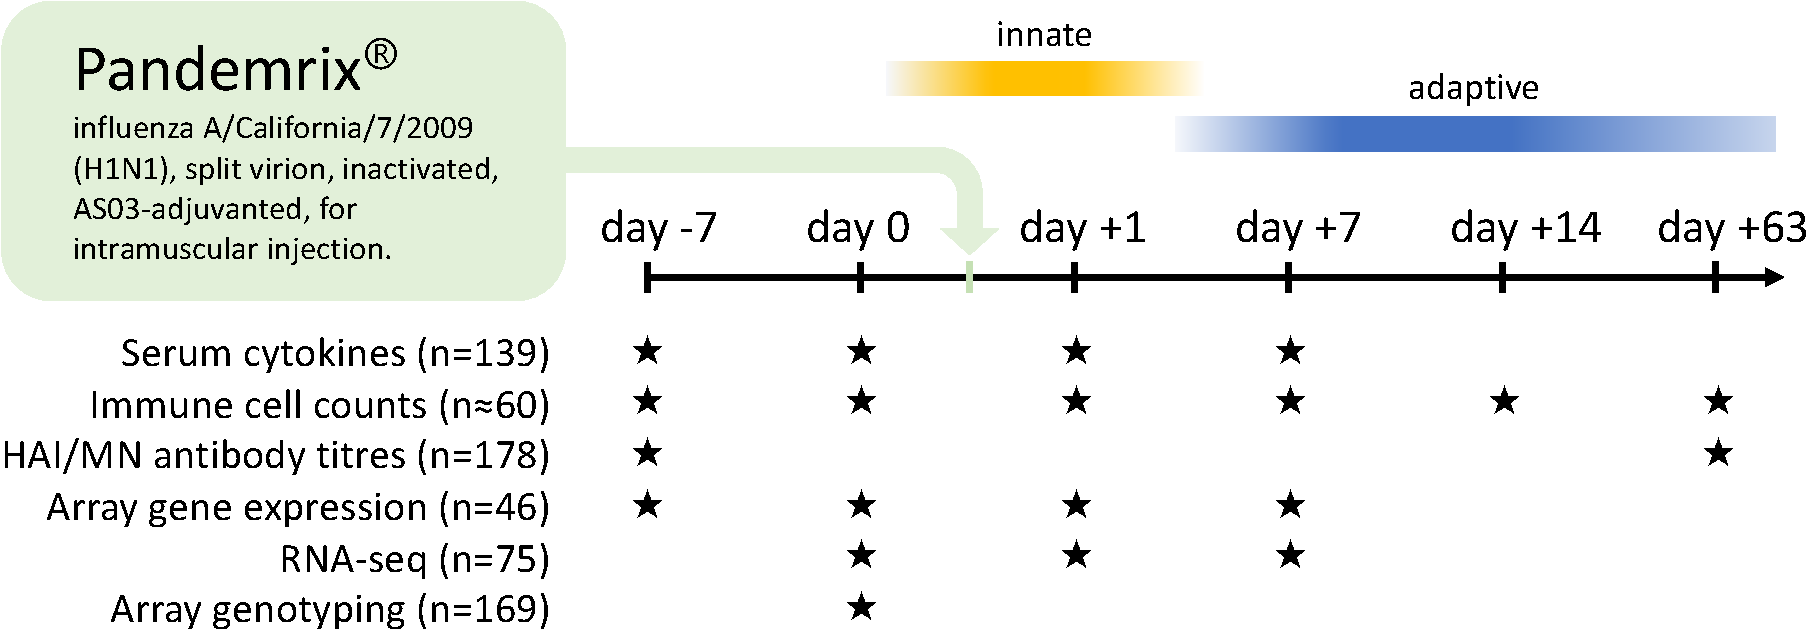
\includegraphics[width=1.0\textwidth]{mainmatter/figures/chapter_02/graphics_ashg19/hird_design-crop.pdf}
    \caption{Data types, timepoints, and sample sizes. Individuals were vaccinated after day 0 sampling. Vaccine-induced antibodies measured by \gls{HAI} and \gls{MN} assays. Array and \gls{RNAseq} gene expression measured in the \gls{PBMC} compartment.}
    \label{fig:hird_design}
\end{figure}

\subsection{Computing baseline-adjusted measures of vaccine-induced antibody response}

In \autocite{sobolev2016AdjuvantedInfluenzaH1N1Vaccination}, Pandemrix responders were defined, according to clinical convention (e.g. \autocite{foodanddrugadministration2007GuidanceIndustryClinical}), as individuals with $\ge$4-fold titre increases in either the \gls{HAI} or \gls{MN} assays.
The responder status for 166 individuals with both \gls{HAI} and \gls{MN} titres available at baseline (day -7) and post-vaccination (day 63) were computed according to this definition.

% \begin{outline}
% \1 Pre-process phenotypes
%     \2 Compute responder status (>= 4-fold in HAI or MN)
%     \2 Compute TRI (based on Bucasas 2009)
%         \3 “We related the change in titer between pre- and postvaccination measurements (response variable) to the prevaccination titer (explanatory variable) using a simple linear model”
%         \3 “We next determined the residuals from the above linear regressions and used them as the input values for the individual response scores.”
%         \3 “we standardized the residuals by dividing by the residual standard deviation for each component”
%             \4 Based on their axis ranges, it appears they are plotting log2(post)-log2(pre)), equivalently log2(post/pre), a.k.a. log2 fold-change; against log2(pre)
%             \4 Note that log2(post-pre) does not make sense mathematically, as post-pre may well be negative
%             \4 The negative relationship indicates lower initial titres are more amenable to high fold-change increases, which is exactly what TRI is designed to correct for
% \end{outline}
However, \autocite{sobolev2016AdjuvantedInfluenzaH1N1Vaccination} noted there was heterogeneity in the baseline titres of non-responders, citing \enquote{glass ceiling} non-responders whose high baseline titres made the fixed 4-fold threshold hard to achieve.\todo{cite appropriate subfigures here}
Dichotomisation of continuous response variables can also result in loss of statistical power \autocite{cohen1983CostDichotomization, fedorov2009ConsequencesDichotomization}.
To address these concerns, I also computed the \gls{TRI} as defined in \textcite{bucasas2011EarlyPatternsGene}.
For each assay, a linear regression was fit with the $\log_2$ fold change $\log_2{\text{day 63}/\text{day -7}}$ as the response, and the $\log_2$ baseline titre $\log_2{\text{day -7}}$ as predictor.
The residuals from the two regressions were each standardized to mean 0 and \gls{SD} 1, then averaged.
The \gls{TRI} expresses a continuous measure of change in antibody titres across both assays post-vaccination, compared to individuals with a similar baseline titre, and remains comparable to the binary 4-fold change definition (\autoref{fig:hird_tri}).\todo{cite appropriate subfigures here}

\begin{figure}
    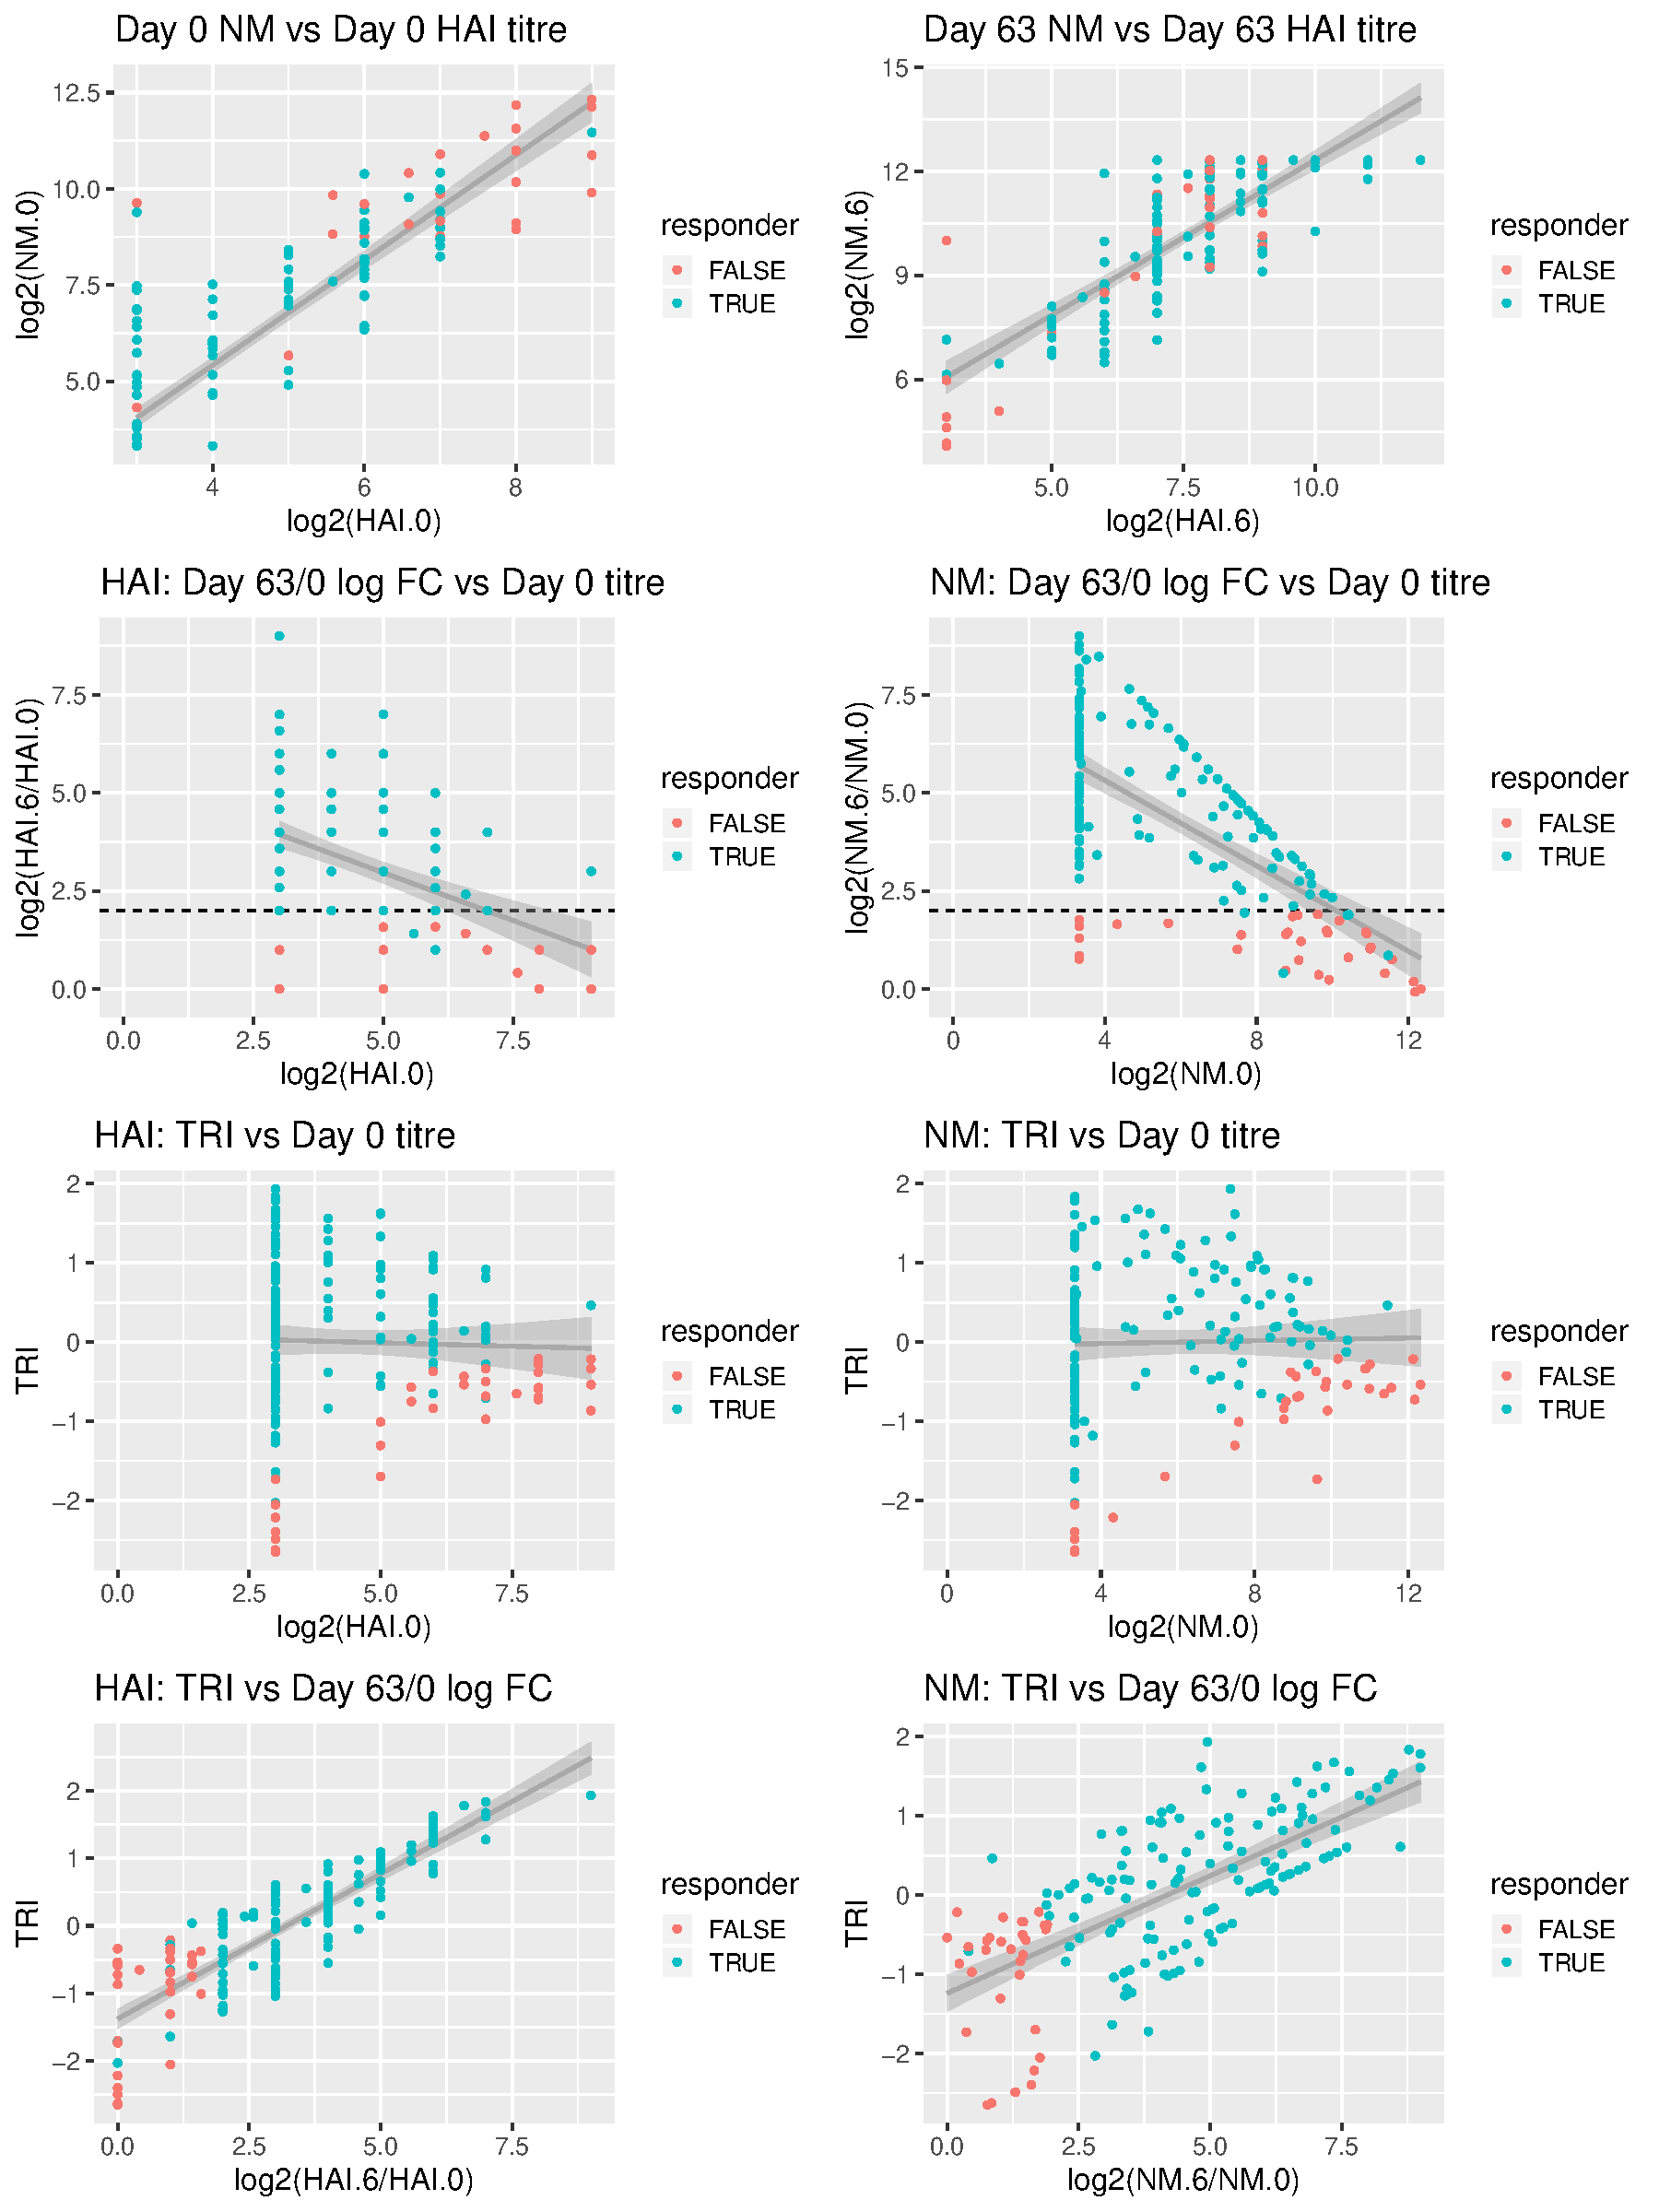
\includegraphics[width=1.0\textwidth]{mainmatter/figures/chapter_02/phenotype_data_setup.tri_comparison.pdf}
    \caption{How TRI corrects fold changes for baseline titre.}
    \label{fig:hird_tri}
\end{figure} 

Descriptive statistics for individuals with both gene expression and antibody titre data are presented in \autoref{tab:hird_table1}.
Although the proportion of responders between array (32/44) and \gls{RNAseq} (59/70) individuals is similar ($p = 0.1551$, Fisher's exact test), the variance of \gls{TRI} in array individuals is higher ($p = 0.0002098$, Levene's test), suggesting more extreme response phenotypes are present (\autoref{fig:hird_phenotypes_by_platform}).

\begin{table}[] 
 \centering 
 \caption{\textbf{Descriptive statistics for individuals with both expression and antibody data.} Values are count and percentage for categorial variables; mean and standard deviation for continuous variables. P values are for the comparison between platforms.}\label{tab:hird_table1}
 \begin{tabular}{ l c c c }
 \toprule
  &   &  \multicolumn{ 2 }{c}{ Platform }\\ 
  & Total & Array & \gls{RNAseq} \\ 
  & n = 114 & n = 44 & n = 70 \\ 
  \midrule
 Gender &   &   &  \\ 
 \hspace{6pt}    F & 72 (63.2\%) & 27 (61.4\%) & 45 (64.3\%)\\ 
 \hspace{6pt}    M & 42 (36.8\%) & 17 (38.6\%) & 25 (35.7\%)\\ 
 Age at vaccination (years)  &   &   &  \\ 
 \hspace{6pt}   & 29.2 (11.8) & 32.9 (14.1) & 26.8 (9.4)\\ 
 Ancestry (self-reported) &   &   &  \\ 
 \hspace{6pt}    Asian & 14 (12.3\%) & 5 (11.4\%) & 9 (12.9\%)\\ 
 \hspace{6pt}    Black/African & 9 (7.9\%) & 4 (9.1\%) & 5 (7.1\%)\\ 
 \hspace{6pt}    Caucasian & 82 (71.9\%) & 33 (75\%) & 49 (70\%)\\ 
 \hspace{6pt}    Latin American & 2 (1.8\%) & 1 (2.3\%) & 1 (1.4\%)\\ 
 \hspace{6pt}    Mixed & 5 (4.4\%) & 1 (2.3\%) & 4 (5.7\%)\\ 
 \hspace{6pt}    Other - Arab & 1 (0.9\%) & 0 (0\%) & 1 (1.4\%)\\ 
 \hspace{6pt}    White Other & 1 (0.9\%) & 0 (0\%) & 1 (1.4\%)\\ 
 log2 day -7 HAI  &   &   &  \\ 
 \hspace{6pt}   & 4.4 (1.8) & 4.2 (1.6) & 4.5 (1.9)\\ 
 log2 day 63 HAI  &   &   &  \\ 
 \hspace{6pt}   & 7.6 (1.8) & 7.4 (2.2) & 7.6 (1.5)\\ 
 log2 HAI fold change  &   &   &  \\ 
 \hspace{6pt}   & 3.2 (1.9) & 3.2 (2.4) & 3.1 (1.6)\\ 
 log2 day -7 MN  &   &   &  \\ 
 \hspace{6pt}   & 6.2 (2.8) & 5.4 (2.4) & 6.6 (3.0)\\ 
 log2 day 63 MN  &   &   &  \\ 
 \hspace{6pt}   & 10.4 (2.0) & 9.5 (2.2) & 10.9 (1.6)\\ 
 log2 MN fold change  &   &   &  \\ 
 \hspace{6pt}   & 4.2 (2.3) & 4.1 (2.6) & 4.3 (2.1)\\ 
 Responder (binary definition) &   &   &  \\ 
 \hspace{6pt}    FALSE & 23 (20.2\%) & 12 (27.3\%) & 11 (15.7\%)\\ 
 \hspace{6pt}    TRUE & 91 (79.8\%) & 32 (72.7\%) & 59 (84.3\%)\\ 
 TRI &   &   &  \\ 
 \hspace{6pt}   & -0.0 (0.9) & -0.2 (1.2) & 0.1 (0.7)\\ 
 \bottomrule
 
 \end{tabular}
 \end{table}


\begin{figure}
    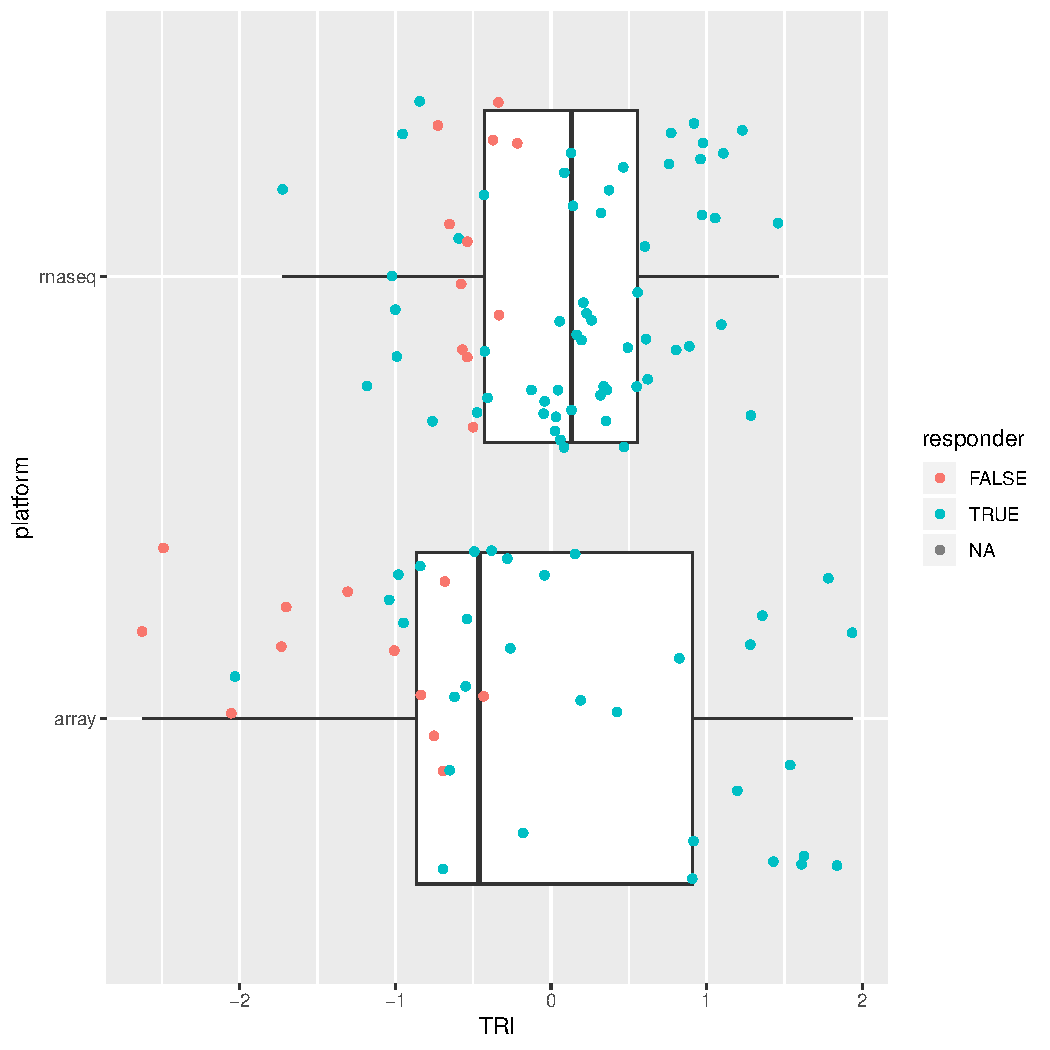
\includegraphics[width=1.0\textwidth,page=1]{mainmatter/figures/chapter_02/compare_phenotype_by_platform.pheno_boxplots.pdf}
    \caption{TRI vs platform}
    \label{fig:hird_phenotypes_by_platform}
\end{figure}

\subsection{Genotype data generation}

\todo{Add to collab note}
DNA was extracted from frozen blood using the Blood and Tissue DNeasy kit (Qiagen), and genotyping was performed using on the Infinium CoreExome-24 BeadChip (Illumina).
In total, 192 samples from 176 patients in the HIRD cohort were genotyped at 550601 markers, including replicate samples submitted for patients where extracted DNA concentrations were low.

\subsection{Genotype data preprocessing}

Using PLINK (v1.90b3w), genotype data underwent the following quality control procedures to remove poorly genotyped samples and markers:
max marker missingness across samples $< 5\%$, 
max sample missingness across markers $< 1\%$, 
max marker heterozygosity rate within 3 standard deviations of the mean (threshold selected visually to exlude outliers, \autoref{fig:hird_genotype_sample_hetRate_missingness}),
% The HWE threshold should depend on the multi-ethnicity of the cohort
removal of markers that deviate from Hardy–Weinberg equilibrium (\texttt{--hwe} option, $\text{p} < 0.00001$).

\begin{figure}
    \includegraphics[width=1.0\textwidth,page=2]{mainmatter/figures/chapter_02/coreex_eQTLflu_20171204.gencall.smajor.impute_sex.qc2.pdf}
    \caption{Sample filters for missingness vs heterozygosity rate.}
    \label{fig:hird_genotype_sample_hetRate_missingness}
\end{figure}

To exclude highly-related individuals and deduplicate replicate samples, pairwise kinship coefficients were computed on \gls{MAF} $< 0.05$ pruned genotypes using KING (v1.4).
For each pair of samples with pairwise kinship coefficient $> 0.177$ (first-degree relatives or closer), the sample with lower marker missingness was selected.

After filtering, 169 samples and 549414 markers remained.

\subsection{Computing genotype \glsfmtshortpl{PC} as covariates for ancestry}

As shown in \autoref{tab:hird_table1}), the \gls{HIRD} cohort is multi-ethnic, hence there is potential for confounding by population structure (sample structure due to genetic ancestry) in expression and genetic association studies \autocite{price2006PrincipalComponentsAnalysis,eu-ahsunthornwattana2014ComparisonMethodsAccount,brown2018ExpressionReflectsPopulation}.
Treating HapMap 3 samples as a reference population where the major axes of variation in genotypes are likely to be ancestry, \gls{PCA} was performed using smartpca (v8000) on \gls{LD}-pruned genotypes (\texttt{PLINK --indep-pairwise 50 5 0.2}).
\gls{HIRD} sample \glspl{PC} were computed by projection onto the HapMap 3 \gls{PCA} eigenvectors.
For non-genotyped individuals, \gls{PC} values were imputed as the mean value for all genotyped individuals with the same self-reported ancestry.
The top \glspl{PC} separate samples of European, African and Asian ancestry (\autoref{fig:hird_genotype_pca_withHapmap}), hence these \glspl{PC} can be used as covariates for ancestry downstream.
\todo{Add Tracy-Widom statistics for PCs}

\begin{figure}
    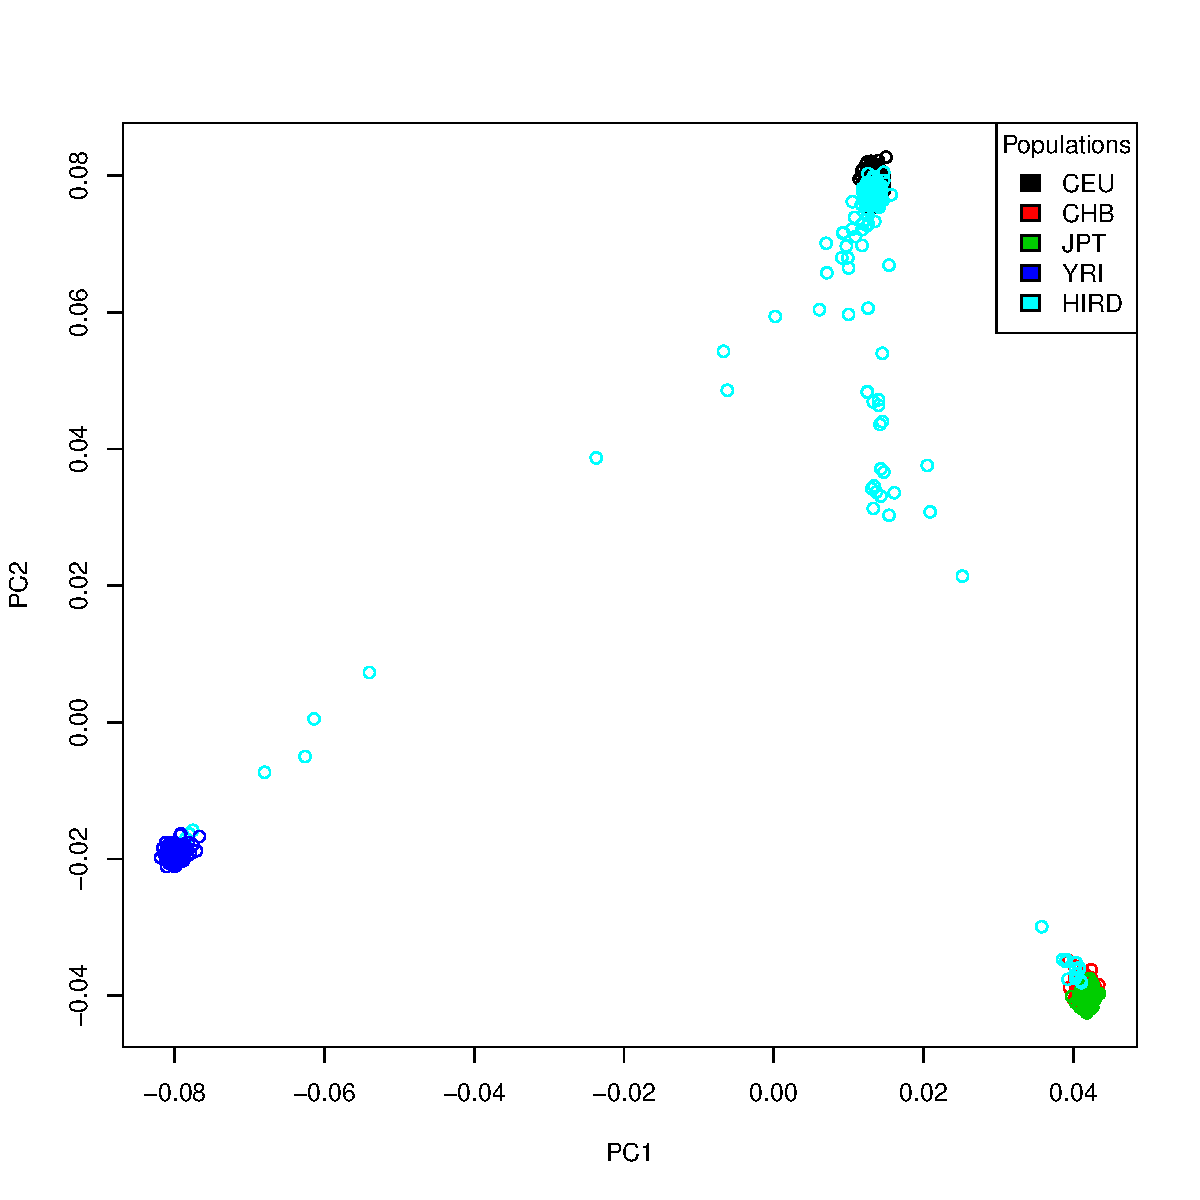
\includegraphics[width=1.0\textwidth]{mainmatter/figures/chapter_02/coreex_eQTLflu_20171204.gencall.smajor.impute_sex.qc3.pruned.hapmap_merged.flipped.pca.evec.pdf}
    \caption{HIRD samples (cyan) projected onto \gls{PC}1 and PC2 axes defined by PCA of HapMap samples. The first two PCs separate European (CEU, upper-right) from Asian (CHB and JPT, lower-right) and African (YRI, lower-left) populations.}
    \label{fig:hird_genotype_pca_withHapmap}
\end{figure}

\subsection{Genotype phasing and imputation}

% 2.	Online imputation service to phase and impute chr 1-22 and X
% 2.1.	Phase with Eagle v2.4 (version in imputation logs.tar.gz)
% 2.2.	Impute with PBWT 3.1-v3.1-2-gbf6ebe2+htslib-1.3.2-199-gec1d68e-dirty (version in vcf header)
% 2.2.1.	Reference fa is human_g1k_v37.fasta (1000 genomes)
% 2.2.2.	X chrom is done in 3 chunks
% 2.2.2.1.	X:1-2699520: impute against reference resources/refs/imputation/hrc.r1.1/pbwt/HRC.r1-1.GRCh37.chrX_PAR1.shapeit3.mac5.aa.genotypes
% 2.2.2.2.	X:2699521-154931043: impute against reference resources/refs/imputation/hrc.r1.1/pbwt/HRC.r1-1.GRCh37.chrX_nonPAR.shapeit3.mac5.aa.genotypes
% 2.2.2.3.	X:154931044-155270560: impute against reference resources/refs/imputation/hrc.r1.1/pbwt/HRC.r1-1.GRCh37.chrX_PAR2.shapeit3.mac5.aa.genotypes
Prior to imputation, 213277 monomorphic markers that provide no information for imputation were removed.
Imputation for the autosomes and X chromosome was conducted using the Sanger Imputation Service\footnote{\url{https://imputation.sanger.ac.uk/}}, which involves pre-phasing with EAGLE2 (v2.4), then imputation with PBWT (v3.1) using the Haplotype Reference Consortium (r1.1) panel.
Markers were lifted-over from GRCh37 to GRCh38 coordinates using CrossMap.
% 4.	Filtering
% 4.1.	BCFTOOLS_INCLUDE="MAF>$MAF_THRESH & F_MISSING<0.05 & FILTER==\"PASS\" & INFO/INFO>0.4"
% 4.2.	Use MAF thresholds 0.05, 0.10, 0.20
Poorly-imputed markers with ($\text{INFO} < 0.4$) or missingness $> 5\%$ were removed, resulting in 40290981 markers.

\subsection{\glsfmtshort{RNAseq} data generation}

Total RNA was extracted from \glspl{PBMC} using the Qiagen RNeasy Mini kit, with on-column DNase treatment.
RNA integrity was checked on the Agilent Bioanalyzer and mRNA libraries were prepared with the KAPA Stranded mRNA-Seq Kit (KK8421), which uses poly(A) selection.
% 7 lanes x 3 plates
To avoid confounding of timepoint and batch effects from pooling, samples were pooled by library prep plate, ensuring libraries from all timepoints of an individual were in the same pool, and then sequenced across multiple lanes as technical replicates (HiSeq 4000, 75bp paired-end).

% To get to cram files:
% From .cram headers:
% 1.	The NextSeq, HiSeq, and NovaSeq Sequencing Systems generate raw data files in binary base call (BCL) format.
% 1.1.	HiSeq Sequencing Control Software (SCS), version HD 3.4.0.38, used for basecalling
% 2.	biobambam2/bamadapterfind: bamdapterfind scans a BAM file for contaminations by sequencing adapters.
% 3.	bambi decode: decode a multiplexed bam file
% 4.	bwa sampe (alignment using BWA-backtrack): alignment to phiX, which is then merged with the original bam
% 5.	pb_calibration/spatial_filter: Identify regions with spatially correlated errors e.g. bubbles, (from aligned BAM files where the read name can be parsed for spatial location) and allow filtering out or marking of the BAM fail bit for reads in those regions.
% 6.	Alignment with tophat 2.0.14
% 6.1.	 --keep-fasta-order --no-sort-bam --output-dir tophat_out_24165_1#10 --mate-inner-dist 100 --num-threads=8 --library-type=fr-firststrand --no-coverage-search --microexon-search --transcriptome-index=/lustre/scratch117/core/sciops_repository/transcriptomes/Homo_sapiens/ensembl_83_transcriptome/GRCh38_15_plus_hs38d1/tophat2/GRCh38_15_plus_hs38d1.known/lustre/scratch117/core/sciops_repository/references/Homo_sapiens/GRCh38_15_plus_hs38d1/all/bowtie2/Homo_sapiens.GRCh38_15_plus_hs38d1.fa
% 7.	Some sort of duplicate marking and filtering (?) using some combination of:
% 7.1.	biobambam/bamsormadup: parallel sorting and duplicate marking
% 7.2.	uk.ac.sanger.npg.picard.AlignmentFilter
% 7.3.	biobambam/bamstreamingmarkduplicates
% 8.	Write .cram files using scramble (cram is a reference-based compression)
% 8.1.	/lustre/scratch117/core/sciops_repository/references/Homo_sapiens/GRCh38_15_plus_hs38d1/all/fasta/Homo_sapiens.GRCh38_15_plus_hs38d1.fa
% 9.	NOTE: Note lots of intermediate biobambam 2.0.76 and scramble processing steps, not all are listed.

\todo{Can add other fastqc plots e.g. kmers, overrepresented seqs, seq length}
% Genomic origin of reads and gene end biases were assessed using Qualimap, after aligning the reads to the human GRCh38_15_plus_hs38d10 reference transciptome using tophat2.
RNA-seq quality metrics were assessed using FASTQC\footnote{\url{https://www.bioinformatics.babraham.ac.uk/projects/fastqc/}} and Qualimap\autocite{okonechnikov2015QualimapAdvancedMultisample}, then visualised with MultiQC\autocite{ewels2016MultiQCSummarizeAnalysis}.
% See log 2017-11-20 for fastqc discussion
Sequence quality was high (\autoref{fig:hird_fastqc_seqQual}), and duplication levels were low (\autoref{fig:hird_fastqc_seqDupe}).
The unimodal GC-content distribution suggested negligible levels of non-human contamination (\autoref{fig:fastqc_gc}).

\begin{figure}
	\centering
	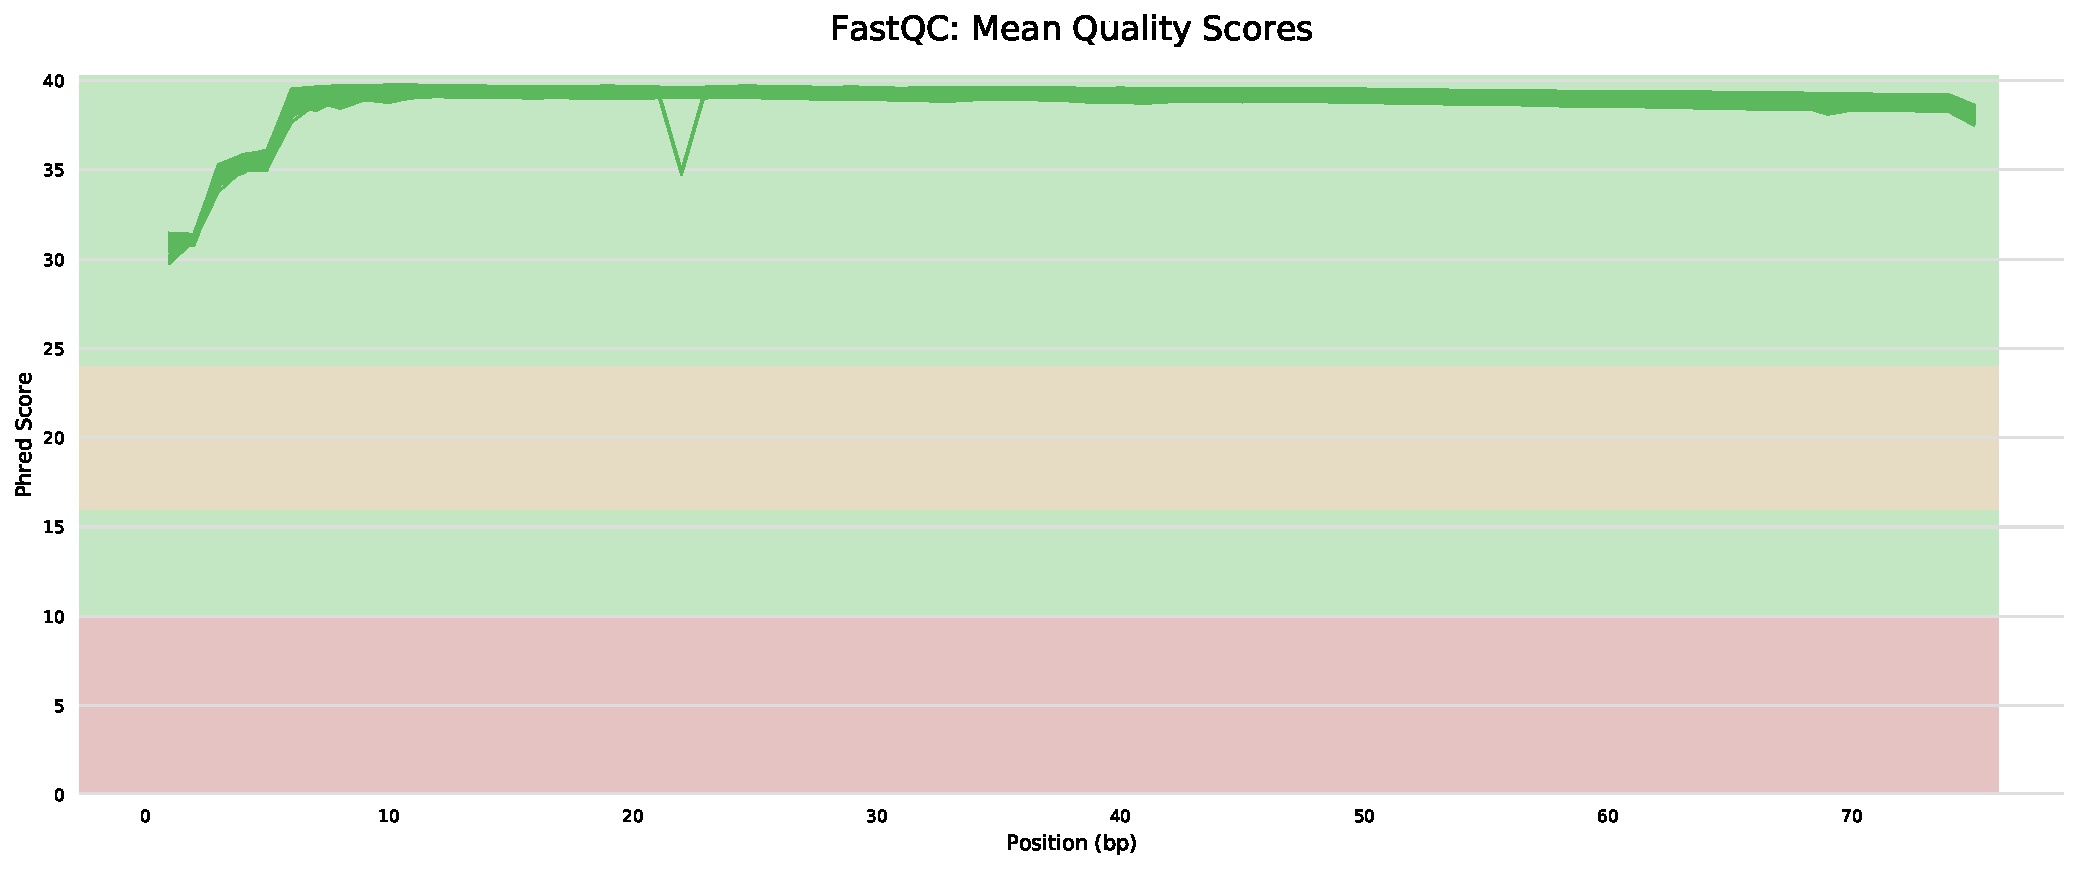
\includegraphics[width=\textwidth]{mainmatter/figures/chapter_02/graphics_firstYearReport/fastqc/mqc_fastqc_per_base_sequence_quality_plot_1.pdf}
    \caption{FastQC sequence quality versus read position for \gls{HIRD} \gls{RNAseq} samples.}
	\label{fig:hird_fastqc_seqQual}
\end{figure}

\begin{figure}
	\centering
	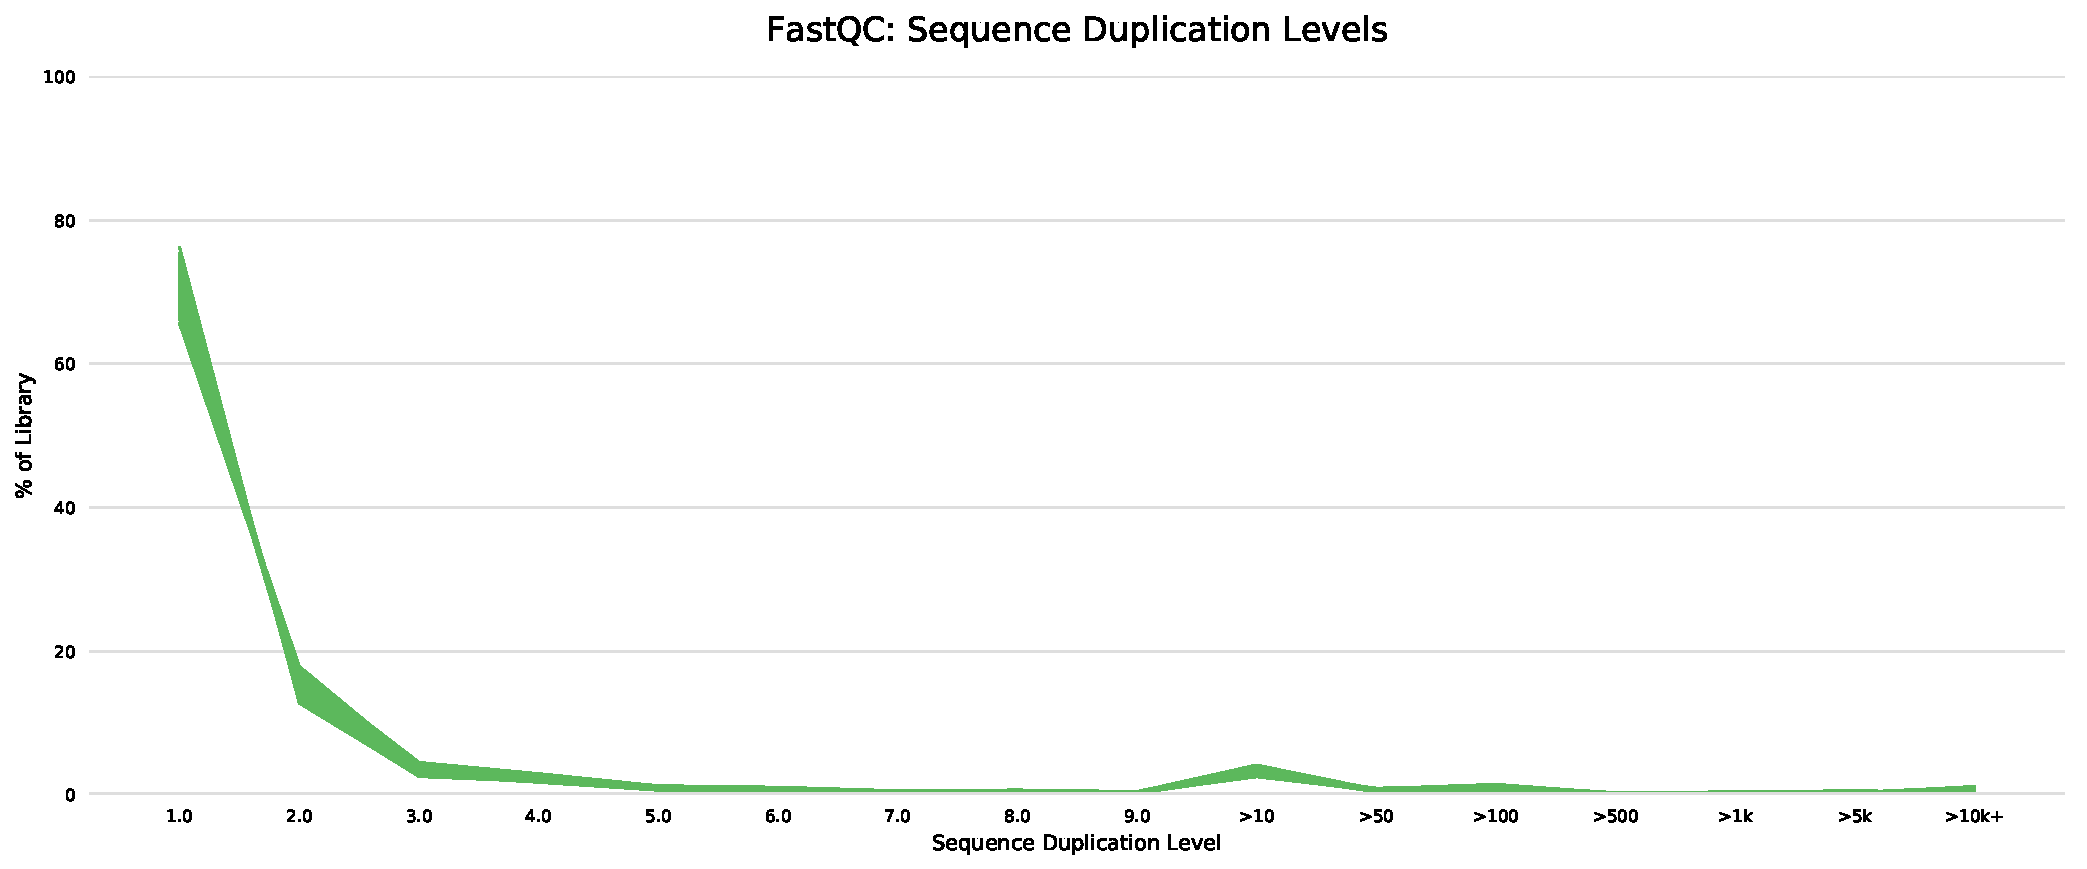
\includegraphics[width=\textwidth]{mainmatter/figures/chapter_02/graphics_firstYearReport/fastqc/mqc_fastqc_sequence_duplication_levels_plot_1.pdf}
	\caption{FastQC sequence duplication levels for \gls{HIRD} \gls{RNAseq} samples.}
	\label{fig:hird_fastqc_seqDupe}
\end{figure}

\begin{figure}
	\centering
	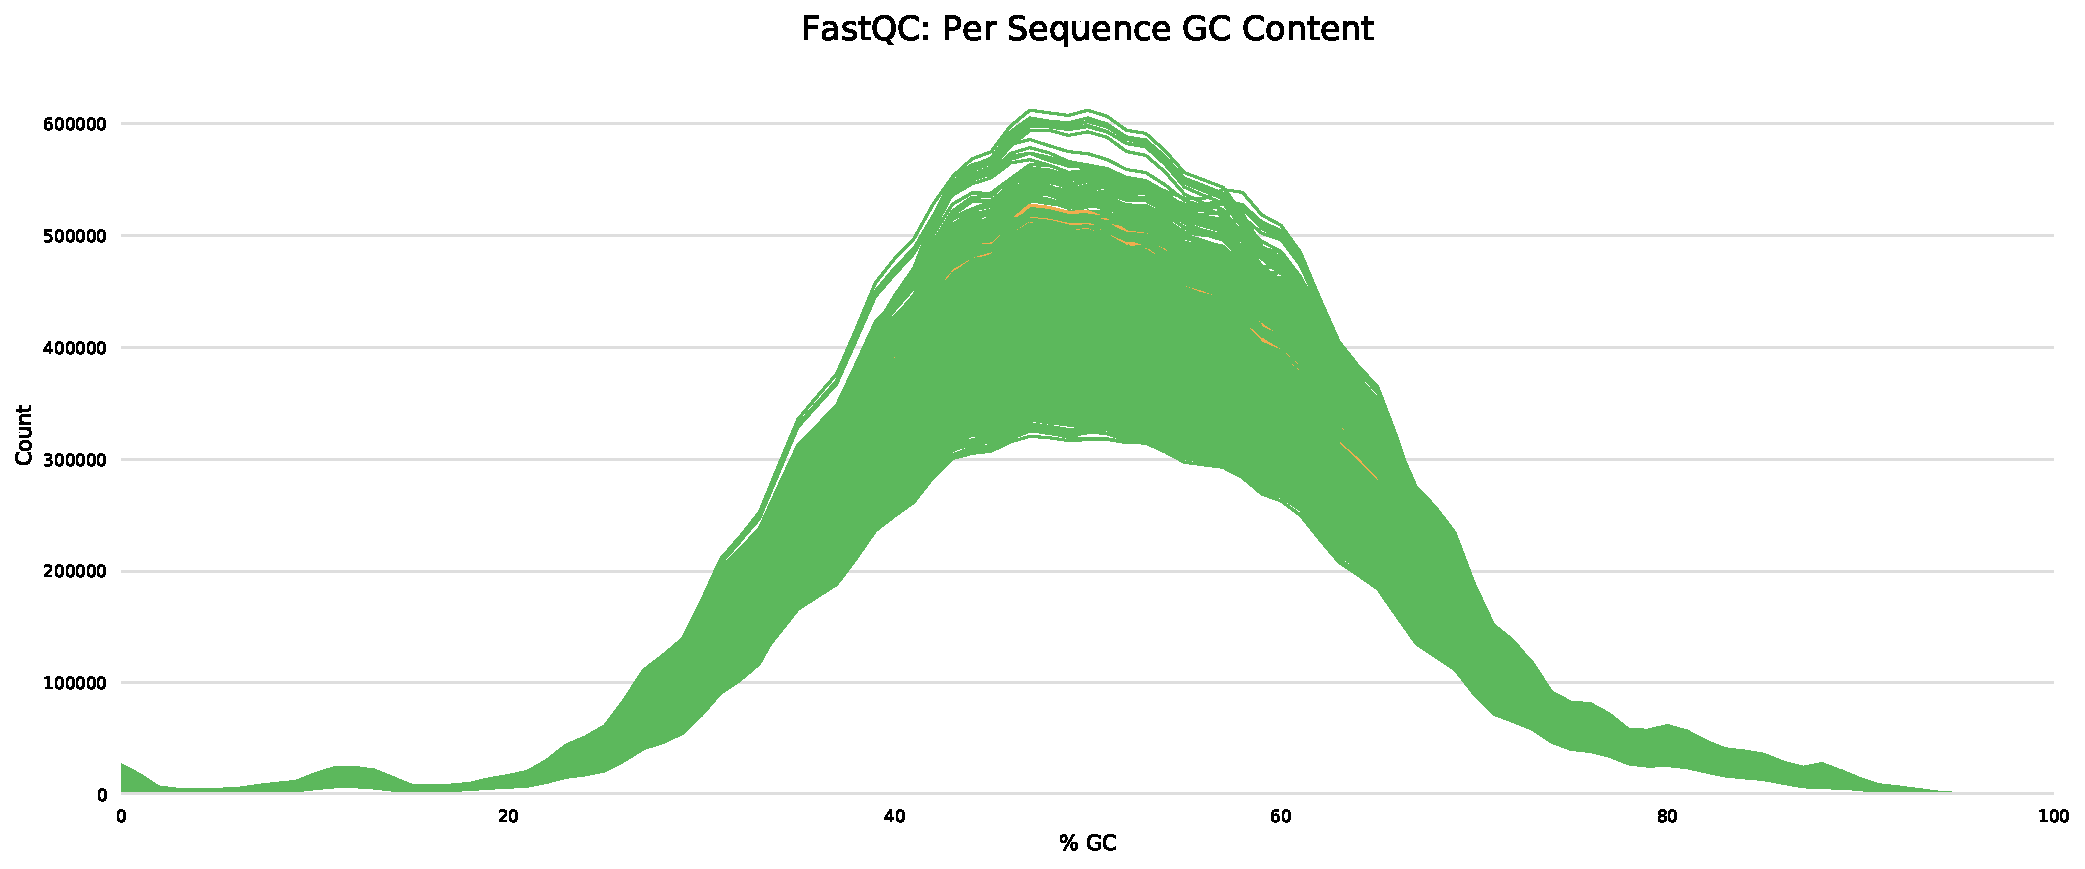
\includegraphics[width=\textwidth]{mainmatter/figures/chapter_02/graphics_firstYearReport/fastqc/mqc_fastqc_per_sequence_gc_content_plot_Counts.pdf}
	\caption{FastQC GC profile for \gls{HIRD} \gls{RNAseq} samples.}
	\label{fig:fastqc_gc}
\end{figure}

\subsection{\glsfmtshort{RNAseq} quantification and filtering}

% 1.	Quantification (Salmon --libType ISR, which is equiv to TopHat -fr-firststrand with paired end data)
% 1.1.	Used index /lustre/scratch117/core/sciops_repository/transcriptomes/Homo_sapiens/ensembl_83_transcriptome/GRCh38_15_plus_hs38
% 1.1.1.	This is GRCh38.p5, Dec 2017, v83; with additional hs38d1: Decoy version 1 for GRCh38
% 1.1.2.	Contains ENST transcript ids
% 1.2.	Output quantifies transcripts in terms of: TPM — This is salmon’s estimate of the relative abundance of this transcript in units of Transcripts Per Million (TPM). TPM is the recommended relative abundance measure to use for downstream analysis.
% 1.2.1.	https://haroldpimentel.wordpress.com/2014/05/08/what-the-fpkm-a-review-rna-seq-expression-units/ TPM = (count/effectiveLength) / sumOverAllTranscripts(count/effectiveLength)
% 1.3.	Note Salmon also takes into account: EffectiveLength — This is the computed effective length of the target transcript. It takes into account all factors being modeled that will effect the probability of sampling fragments from this transcript, including the fragment length distribution and sequence-specific and gc-fragment bias (if they are being modeled).
% 2.	Gene-level regeneration of counts (tximport)
% 2.1.	“generate estimated counts using abundance estimates scaled up to library size (scaledTPM)”
% 2.1.1.	Note, we do not scale for gene length, that would be lengthScaledTPM. Hence the generated counts remain length-corrected.
% 2.2.	Summarizes using a mapping of ENST to ENSG, generated from /lustre/scratch117/core/sciops_repository/transcriptomes/Homo_sapiens/ensembl_83_transcriptome/GRCh38_15_plus_hs38d1/gtf/ensembl_83_transcriptome-GRCh38_15_plus_hs38d1.gtf
% 2.3.	Counts from all lanes of a sample are summed
% 3.	GC bias, length bias, mappability
% 3.1.	Length bias only affects RNAseq: somewhat alleviated by Salmon using effective length
% 3.2.	GC bias affects both technologies: somewhat alleviated by Salmon using effective length (see the salmon paper)
% 3.3.	Mappability has not been considered
\todo{add software versions}
Reads were quantified against the Ensembl reference transcriptome (GRCh38) using Salmon\autocite{patro2017SalmonProvidesFast} in quasi-mapping-based mode, which internally accounts for transcript length and GC composition.
% https://www.biostars.org/p/304552/
To combine technical replicates, as the sum of Poisson distributions remains Poisson-distributed, counts for technical replicates were summed for each sample.
% Also see:
%
% https://genomebiology.biomedcentral.com/articles/10.1186/s13059-016-0881-8
% "While some authors will argue that as few as five million mapped reads are sufficient to quantify accurately medium to highly expressed genes in most eukaryotic transcriptomes, others will sequence up to 100 million reads to quantify precisely genes and transcripts that have low expression levels [7]."
%
% https://genome.ucsc.edu/ENCODE/protocols/dataStandards/ENCODE_RNAseq_Standards_V1.0.pdf
% 2. Sequencing depth.
% The amount of sequencing needed for a given sample is determined by the goals of the experiment and the nature of the RNA sample.
% Experiments whose purpose is to evaluate the similarity between the transcriptional profiles of two polyA+ samples may require only modest depths of sequencing (e.g. 30M pair-end reads of length > 30NT, of which 20-25M are 3mappable to the genome or known transcriptome, Experiments whose purpose is discovery of novel transcribed elements and strong quantification of known transcript isoforms requires more extensive sequencing.
% The ability to detect reliably low copy number transcripts/isoforms depends upon the depth of sequencing and on a sufficiently complex library.
% For experiments from a typical mammalian tissue or in which sensitivity of detection is important, a minimum depth of 100-200 M 2 x 76 bp or longer reads is currently recommended.
The mean number of mapped read pairs per sample after summing was 27.09 million read pairs (range 20.24-39.14 million), representing a mean mapping rate of 80.73\% (range 75.57-90.10\%), comfortably within sequencing depth recommendations for \gls{DGE} experiments\autocite{liu2014RNAseqDifferentialExpression}.
Relative transcript abundances were summarised to Ensembl gene-level count estimates using tximport to improve statistical robustness and interpretability\autocite{soneson2016DifferentialAnalysesRNAseq}.

% 5.	Pre-process RNA-seq expression data
% 5.1.	Pull in tximport counts
% 5.1.1.	60675 loci, 223 samples
% 5.2.	Add gene annotation based on EnsDb.Hsapiens.v86
% 5.3.	Low-count filtering (>0.5 CPM in 10% of 223 samples i.e. 22 samples)
% Max zero prop: need to be stringent as limma doesn't account for neg bin
% 5.4.	Remove globin genes and short non-coding RNAs
% 5.4.1.	Human globins: https://en.wikipedia.org/wiki/Globin#Examples
% 5.4.2.	Short non-coding GENEBIOTYPES: https://www.gencodegenes.org/pages/biotypes.html
% 5.5.	NOTE: we have not yet removed GENEBIOTYPE=NA. These may be retired ids.
Genes with short noncoding RNA biotypes \footnote{miRNA, miRNA\_pseudogene, miscRNA, miscRNA pseudogene, Mt rRNA, Mt tRNA, rRNA, scRNA, snlRNA, snoRNA, snRNA, tRNA, tRNA\_pseudogene. \url{https://www.ensembl.org/Help/Faq?id=468}} were removed, as they are generally not polyadenylated, and expression estimates can be biased by misassignment of counts from overlapping protein-coding or lncRNA genes\autocite{zhao2018EvaluationTwoMain}.
% Also, they can be shorter than the 75 bp read length
Globin genes, which are highly expressed in erythrocytes and reticulocytes, cell types expected to be depleted in \gls{PBMC} \autocite{min2010VariabilityGeneExpression}, were also removed.
Given the proportion of removed counts at this stage was low most samples (\autoref{fig:hird_shortncRNA_and_globins}), poly(A) selection and \gls{PBMC} isolation procedures were deemed to be efficient.

\begin{figure}
    \centering
    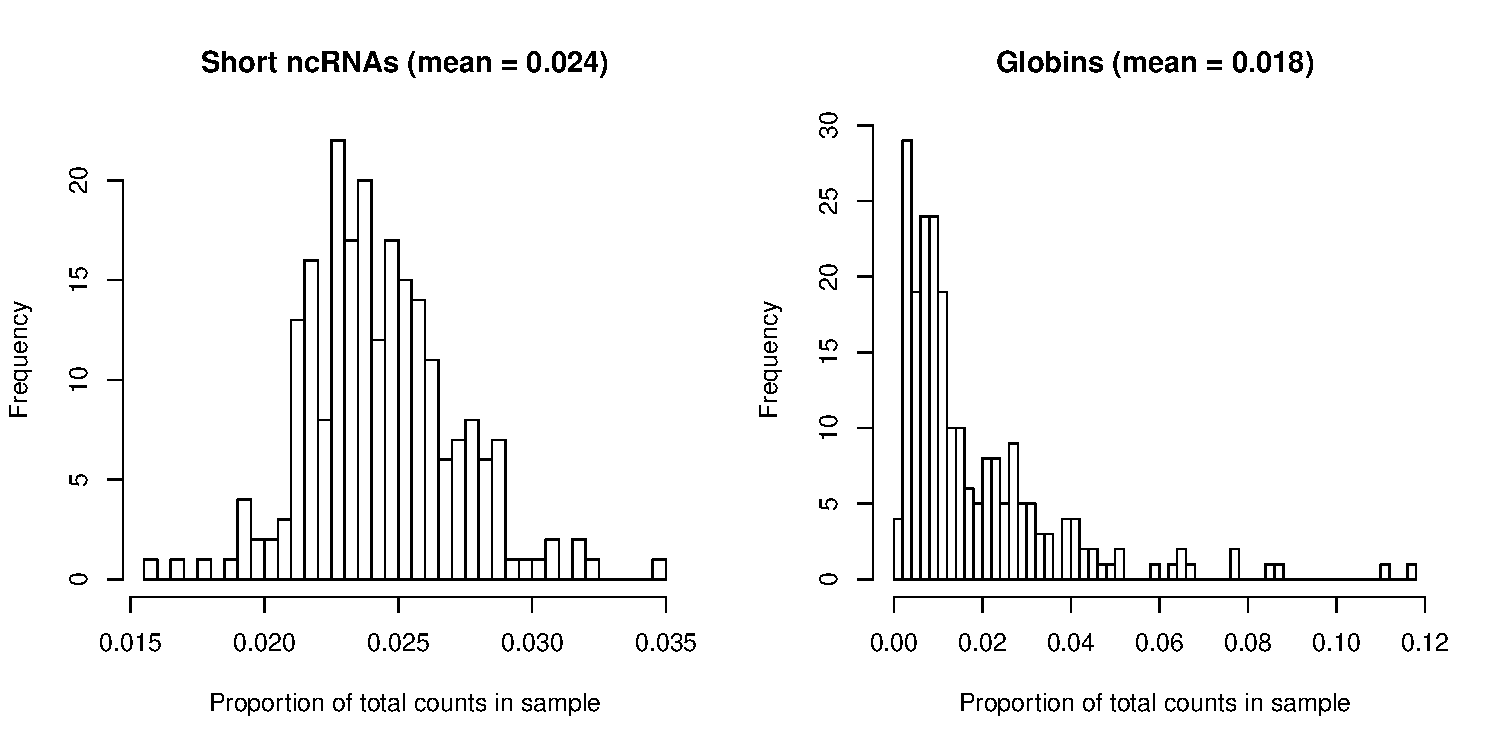
\includegraphics[width=1.0\textwidth, page=1]{mainmatter/figures/chapter_02/rnaseq_data_setup.per_sample.short_ncRNA_globin_levels_hist.pdf}
    \caption{Distribution of short ncRNA and globin counts as a proportion of total counts in \gls{RNAseq} samples.}
    \label{fig:hird_shortncRNA_and_globins}
\end{figure}

Many of the genes in the reference transcriptome are not expressed in \gls{PBMC} (\autoref{fig:hird_rnaseq_filtering_zeroProp}), and many genes are expressed at counts too low for statistical analysis of \gls{DGE}
Genes were further filtered to require detection (non-zero expression) in at least 95\% of samples, and a minimum of 0.5 \gls{CPM} in at least 20\% of samples.
The 0.5 \gls{CPM} threshold was chosen to correspond to approximately 10 counts in the smallest library, where 10-15 counts is a rule of thumb for considering a gene to be robustly expressed \autocite{chen2016ReadsGenesPathways}.
The change in the distribution of gene expressions among samples before and after filtering shows a substantial number of low expression genes are removed (\autoref{fig:hird_rnaseq_cpm_filtering}).

\begin{figure}
    \centering
    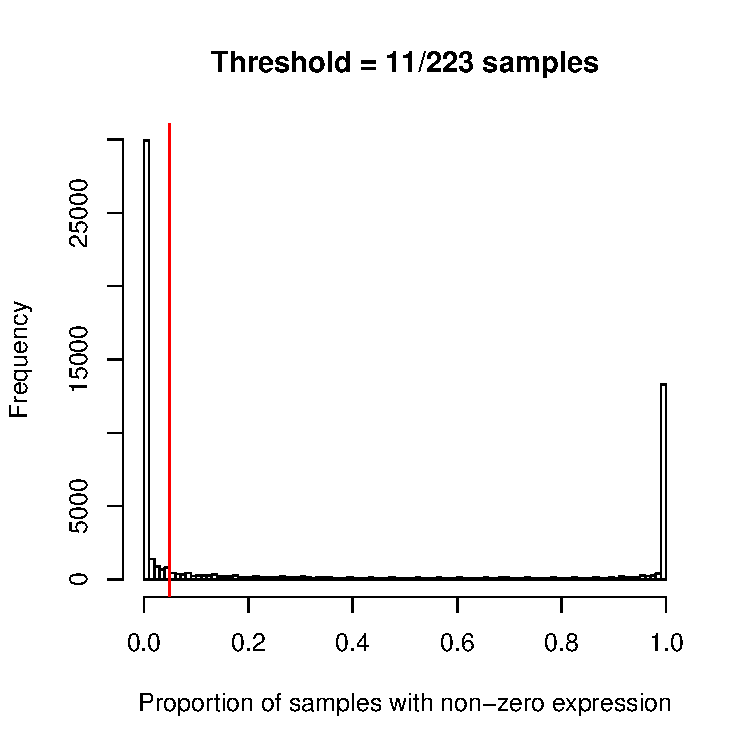
\includegraphics[width=0.6\textwidth, page=1]{mainmatter/figures/chapter_02/rnaseq_data_setup.gene_zero_prop.pdf}
    \caption{Proportion of samples in which genes are detected with non-zero counts. Vertical line shows 5\% threshold.}
    \label{fig:hird_rnaseq_filtering_zeroProp}
\end{figure}

\begin{figure}
    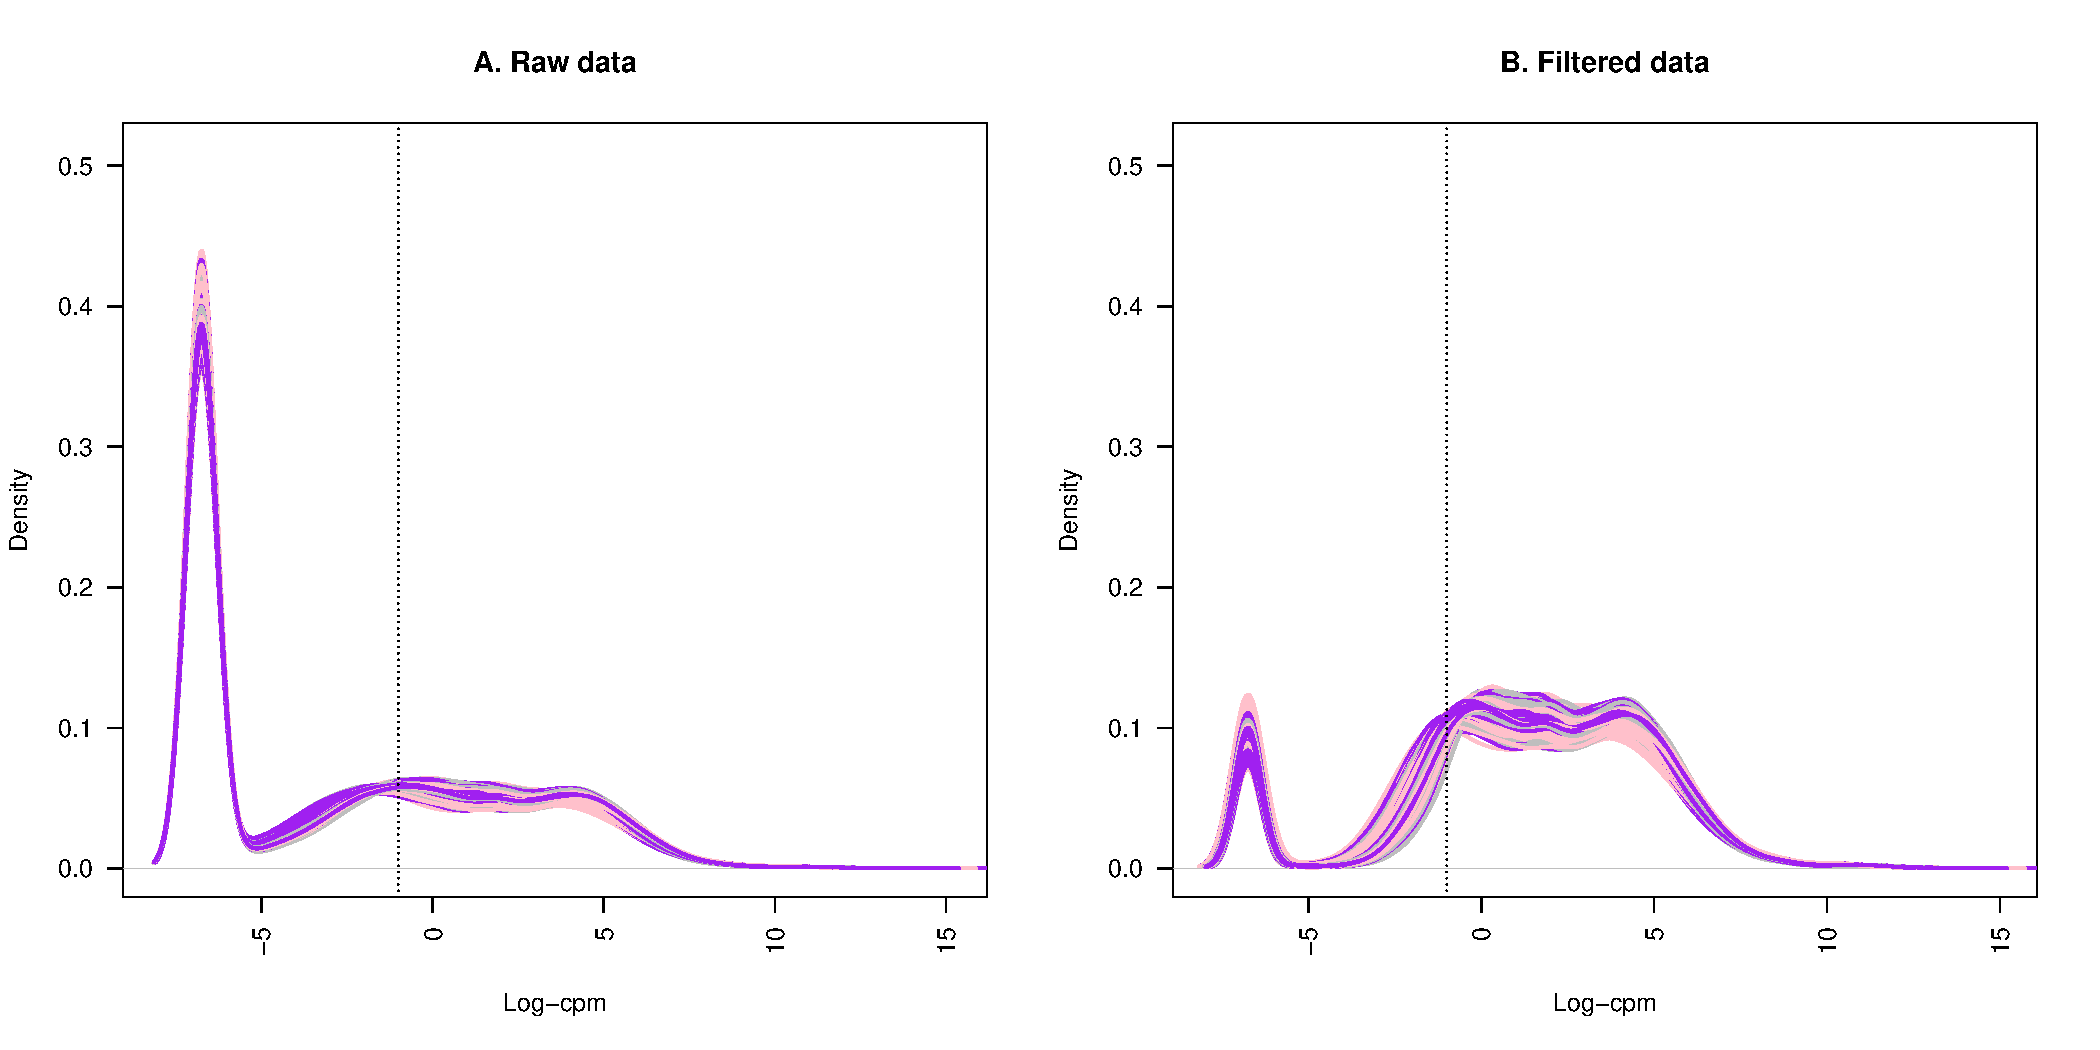
\includegraphics[width=1.0\textwidth]{mainmatter/figures/chapter_02/rnaseq_data_setup.sample_cpm_density_filtered.pdf}
    \caption{Distribution of gene expressions for sample before and after filtering low expression genes. Vertical line shown at log(0.5) \gls{CPM}.}
    \label{fig:hird_rnaseq_cpm_filtering}
\end{figure}

After the application of all filters, expression values were available for 21626 genes over 223 samples (75/75 individuals on day 0, 73/75 on day 1, and 75/75 on day 7).

\subsection{Array data preprocessing}

% 6.	Pre-process microarray expression data
% 6.1.	Annotate Entrez and ENS ids using hgug4112a.db
% 6.1.1.	The chip is single-channel “Agilent-014850 Whole Human Genome Microarray 4x44K G4112F”
% 6.1.2.	Apparently fine to use 4112A db for 4112F https://support.bioconductor.org/p/73193/
% 6.2.	Redefine responder phenotype to be consistent with RNA-seq and Sobolev paper (>= 4-fold in HAI or MN)
% 6.3.	Background correction: limma::backgroundCorrect(x, method="normexp")
% 6.3.1.	Background comes from non-specific binding
% 6.3.2.	Pipeline from the Agi4x44PreProcess Bioconductor package (deprecated)
% 6.3.3.	Notes on Edwards: https://academic.oup.com/bioinformatics/article/23/20/2700/230165#2633725
% 6.3.3.1.	“adjusts the foreground intensities by subtracting the background when the difference between the foreground and background is larger than a small threshold value. When the difference is less than the threshold, subtraction is replaced by a smooth monotonic function.“
% 6.3.3.2.	May be preferred over normexp in our case due to “Question: Compressed boxplots after 'normexp+offset' background correction of Agilent one color microarrays in LIMMA“ https://support.bioconductor.org/p/46485/
% 6.3.3.3.	Example of Edwards used over normexp for Agilent arrays: “Modified least-variant set normalization for miRNA microarray” https://www.ncbi.nlm.nih.gov/pmc/articles/PMC2995391/
% 6.3.3.4.
% 6.3.4.	Notes on normexp:
% 6.3.4.1.	This function is designed to produce positive corrected intensities.
% 6.3.4.1.1.	“If the "normexp" method is selected, then a convolution of normal and exponential distributions is fitted to the foreground intensities using the background intensities as a covariate, and the expected signal given the observed foreground becomes the corrected intensity.”
% 6.3.4.1.2.	https://www.ncbi.nlm.nih.gov/pmc/articles/PMC2648902/ “A method normexp was introduced which models the observed intensities as the sum of exponentially distributed signals and normally distributed background values”
% 6.3.4.2.	[…] an offset value (normally 50) is used. This offset adds a constant to the intensities before log-transforming, so that the log ratios are shrunk towards zero at the lower intensities.
% 6.3.4.3.	The optimal choice for the offset is the one which makes the variability of the log-ratios as constant as possible across the range of intensity values (Smyth, G. in BioC mailing List, https://stat.ethz.ch/pipermail/bioconductor/2006-April/012554.html ).
% 6.3.5.	Choice of offset: https://academic.oup.com/nar/article/38/22/e204/1049223#93002104
% 6.3.5.1.	Adding an offset to the intensities before log transformation not only was found to lower the variance (improve precision) but also to compress the fold-change range and increase bias. In other words, offsets decrease noise but increase bias.
% 6.3.5.2.	The normexp by control (neqc) algorithm […] For routine practical use, we recommend modest offsets for Illumina data in the range of 10–50, which minimize the bias while still delivering a benefit in terms of FDR. Offsets of 16–50 have been used in a number of biological studies (10,13,16). These results remain essentially unchanged whether or not control probes are used […]  The default offset is 16, which seems generally to give good results on recent versions of human and mouse Illumina arrays.
% No need for normalizeWithinArrays in 2 color.
% 6.4.	Between-sample normalization: Limma::normalizeBetweenArrays(y, method="quantile")
% Why quantile normalise arrays? "A comparison of normalization methods for high density oligonucleotide array data based on variance and bias"
% 6.4.1.	Note that we omit any normalize within arrays procedures, as this is a single-channel array
% 6.4.2.	Normalization is the attempt to compensate for systematic technical differences between chips
% 6.4.3.	Uses https://www.rdocumentation.org/packages/limma/versions/3.28.14/topics/normalizeQuantiles
% 6.4.3.1.	“Each quantile of each column is set to the mean of that quantile across arrays. The intention is to make all the normalized columns have the same empirical distribution. This will be exactly true if there are no missing values and no ties within the columns: the normalized columns are then simply permutations of one another.”
% 6.4.4.	Also see this “StatQuest: Quantile Normalization” https://www.youtube.com/watch?v=ecjN6Xpv6SE
% 6.4.5.	This also does a log2 transform, so final units are normalized log2 intensity

Single-channel Agilent 4x44K microarray (G4112F) data for 173 samples from \autocite{sobolev2016AdjuvantedInfluenzaH1N1Vaccination} were downloaded from \url{https://www.ebi.ac.uk/arrayexpress/experiments/E-MTAB-2313/}.
% Actually uses:
% The so-called glog2 (short for generalised logarithm) is a function that is like the logarithm (base 2) for large values (large compared to the amplitude of the background noise), but is less steep for smaller values.
VSN\autocite{huber2002VarianceStabilizationApplied} was used to perform background correction for non-specific hybridisation, between-array normalisation, and variance-stabilisation of intensity values, resulting in expression values on a $\log_2$ scale.

% 6.5.	Summarise probes (into loci): WGCNA::collapseRows(rowGroup=Ensembl ID, method="MaxMean", connectivityBasedCollapsing=FALSE)
% 6.5.1.	https://www.ncbi.nlm.nih.gov/pmc/articles/PMC3166942/
% 6.5.1.1.	“For example, we find that in most microarray experiments performed on brain tissue it is best to choose the probe with the maximum mean expression per gene, whereas when choosing a single gene to represent a co-expression module, the optimal collapsing method depends on the goal of the analysis.”
% 6.5.1.2.	“In the case of collapsing probes to their respective gene symbols, for example, we find that the 1.max strategy (implemented by setting method = "MaxMean" and connectivityBasedCollapsing = FALSE) produces the most robust results.”
% 6.5.1.3.	i.e. choose the probe with the highest mean of expression over the samples
Most genes are covered by multiple array probes; 31208 probes were collapsed into 18216 Ensembl genes using by selecting the probe with the highest mean intensity for each gene (WGCNA::collapseRows, using the MaxMean method recommended for probe to gene collapsing)\autocite{miller2011StrategiesAggregatingGene}.
While it would be optimal to select a collapsing method to maximise the concordance between array and \gls{RNAseq} expression values, there were no samples assayed by both platforms in the \gls{HIRD} dataset.
\todo{standardise form here. final sentence at end of each preprocessing should be n genes x samples x units}

% \begin{figure}
%     \centering
%     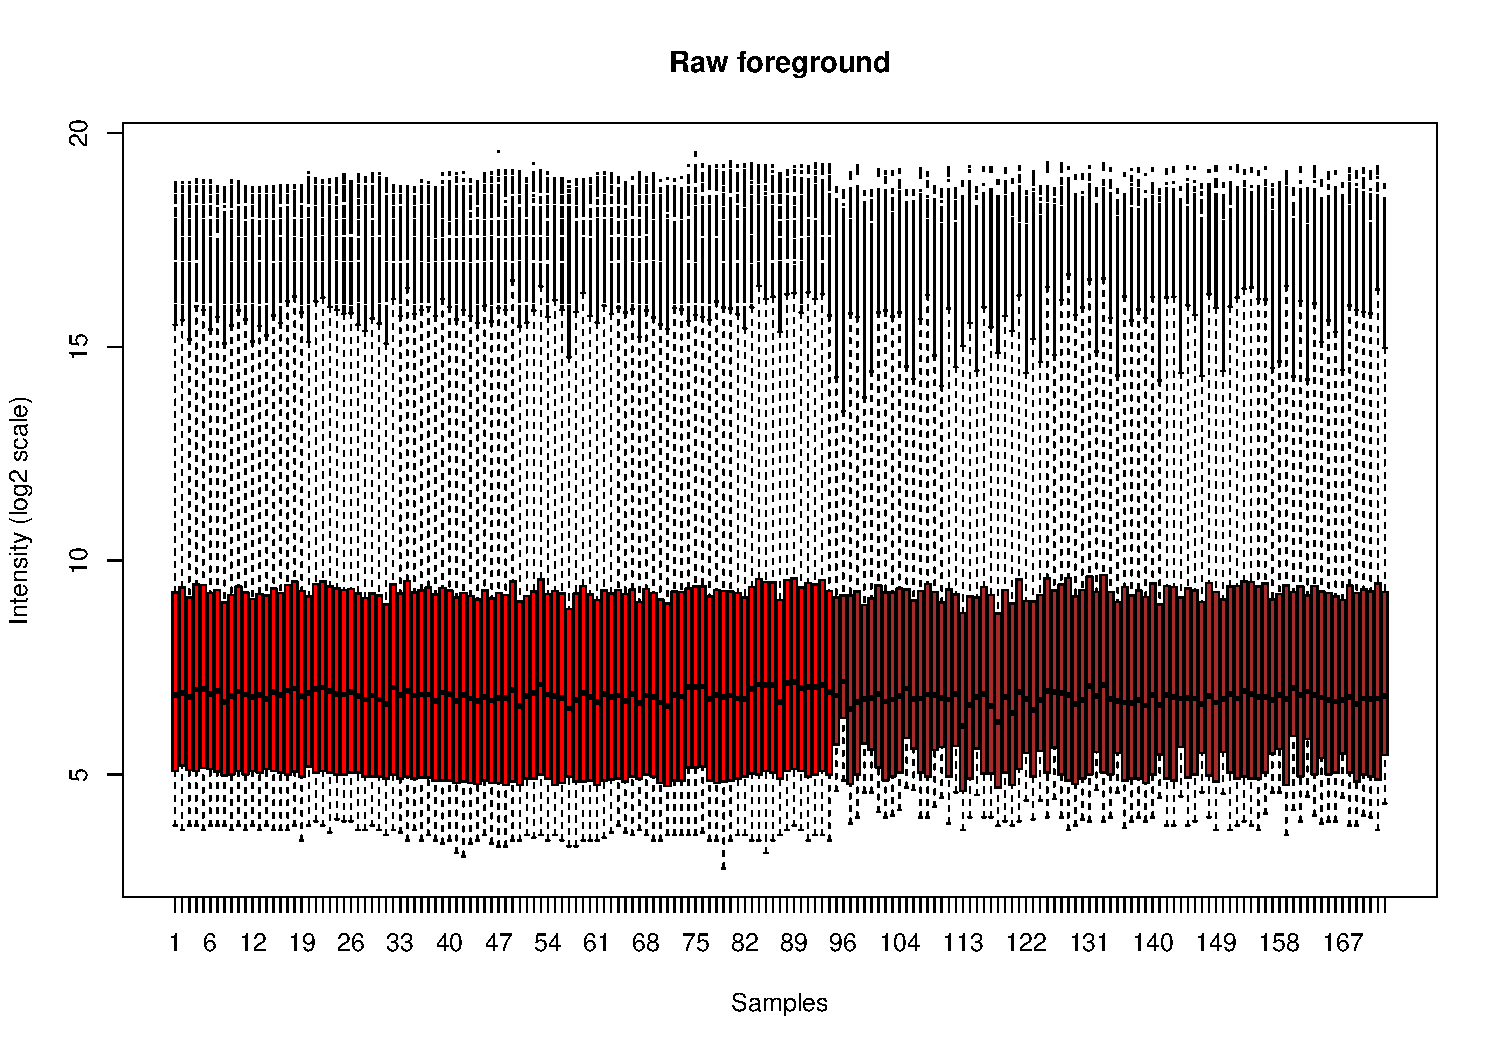
\includegraphics[width=1.0\textwidth,page=1]{mainmatter/figures/chapter_02/array_data_setup.array_intensity_boxplots.pdf}
%     \caption{Raw array intensities.}
%     \label{fig:hird_array_boxplots_raw}
% \end{figure}
%
% \begin{figure}
%     \centering
%     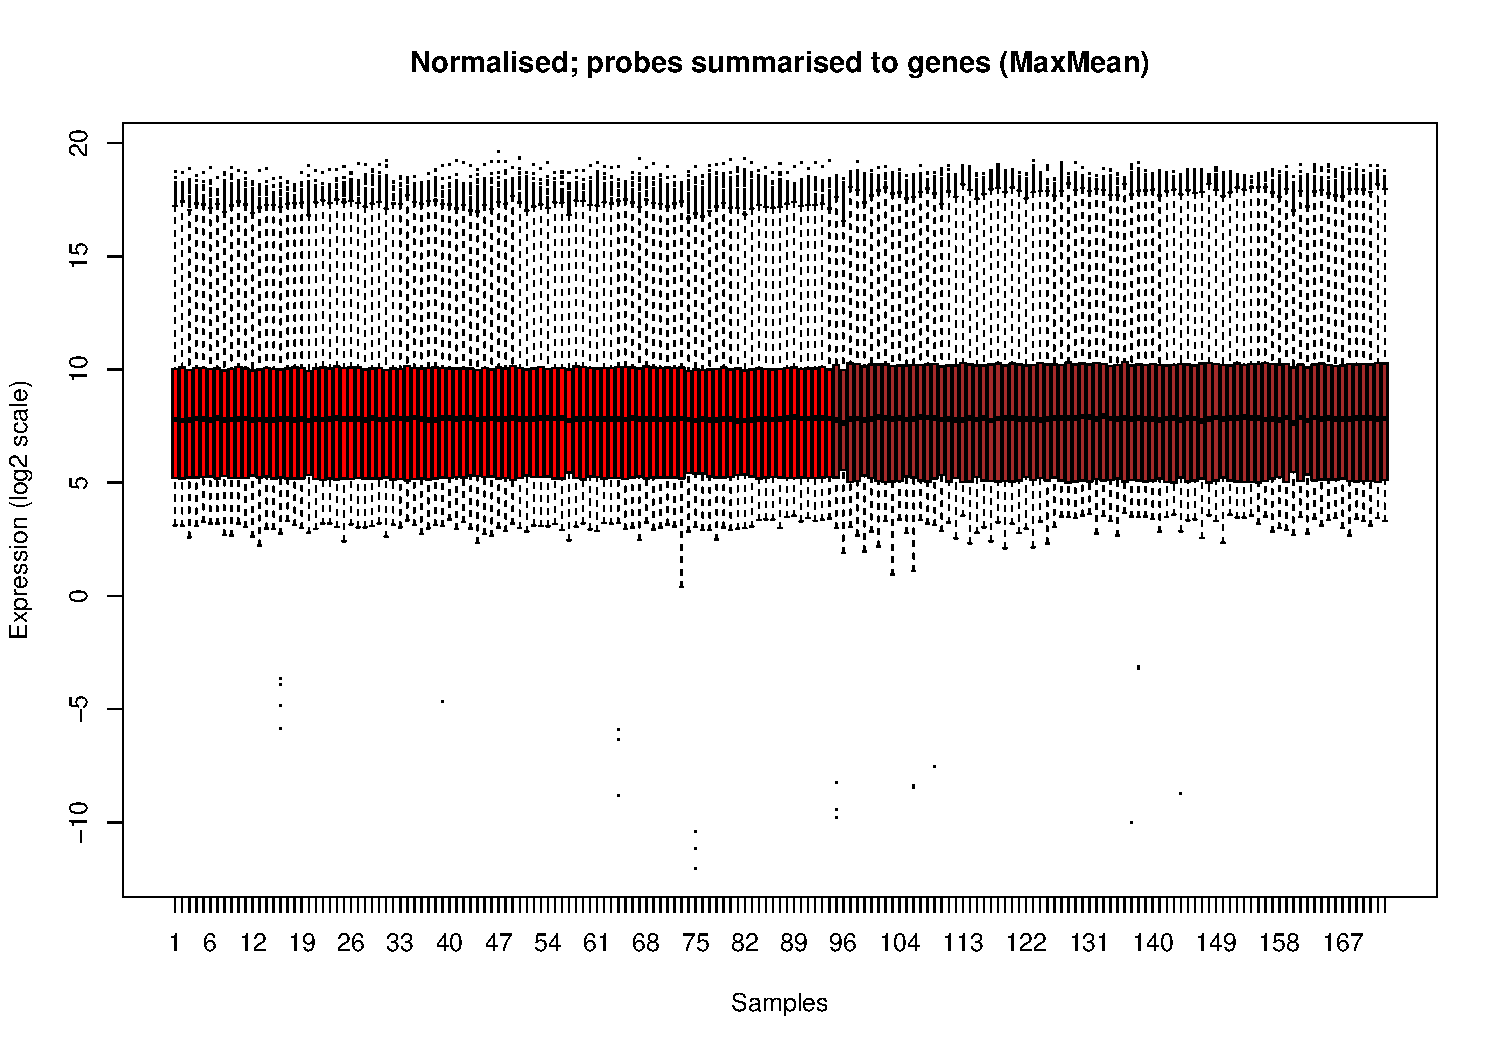
\includegraphics[width=1.0\textwidth]{mainmatter/figures/chapter_02/array_data_setup.array_intensity_boxplots.MaxMean.pdf}
%     \caption{Array intensity estimates after VSN normalisation and collapsing of probes to genes.}
%     \label{fig:hird_array_boxplots_MaxMean}
% \end{figure}

\subsection{\Glsfmtlong{DGE}}

\gls{PCA} of the expression data reveals although samples separate by experimental timepoint along \gls{PC}3 (\autoref{fig:hird_expression_pcs}d), measurement platform is by far the largest source of variation, and a batch effect exists within the array data (\autoref{fig:hird_expression_pcs}a).
% Also see:
% Wang, C., Gong, B., Bushel, P. R., Thierry-Mieg, J., Thierry-Mieg, D., Xu, J., Fang, H., Hong, H., Shen, J., Su, Z., Meehan, J., Li, X., Yang, L., Li, H., Łabaj, P. P., Kreil, D. P., Megherbi, D., Gaj, S., Caiment, F., … Tong, W. (2014). The concordance between RNA-seq and microarray data depends on chemical treatment and transcript abundance. Nature Biotechnology, 32(9), 926–932. https://doi.org/10.1038/nbt.3001
%
% The CBM paper intro has a good summary too. https://www.ncbi.nlm.nih.gov/pmc/articles/PMC5510692/
The large platform effect likely stems from fundamental technological differences in how each platform measures expression.
For example, arrays suffer from ratio compression due to cross-hybridisation\autocite{draghici2006ReliabilityReproducibilityIssues}.
\gls{RNAseq} has a higher dynamic range, resulting less systematic bias at low expression levels, but estimates are more sensitive to changes in depth than array estimates are to changes in intensity \autocite{robinson2015NestedParallelExperiment}.
There are also differences in the statistical models behind expression quantification, as described above\todo{cite relevant preprocessing sections}.

Despite the shortcomings of array data detailed above, the array dataset tends to contain individuals with more extreme antibody response phenotypes (\autoref{fig:hird_phenotypes_by_platform}), and hence the data should not be excluded.
Given the magnitude of the platform effect, I concluded that the appropriate approach should be a two-stage approach that integrates per-platform \gls{DGE} effect estimates while accounting for between-platform heterogeneity.

\begin{figure}
    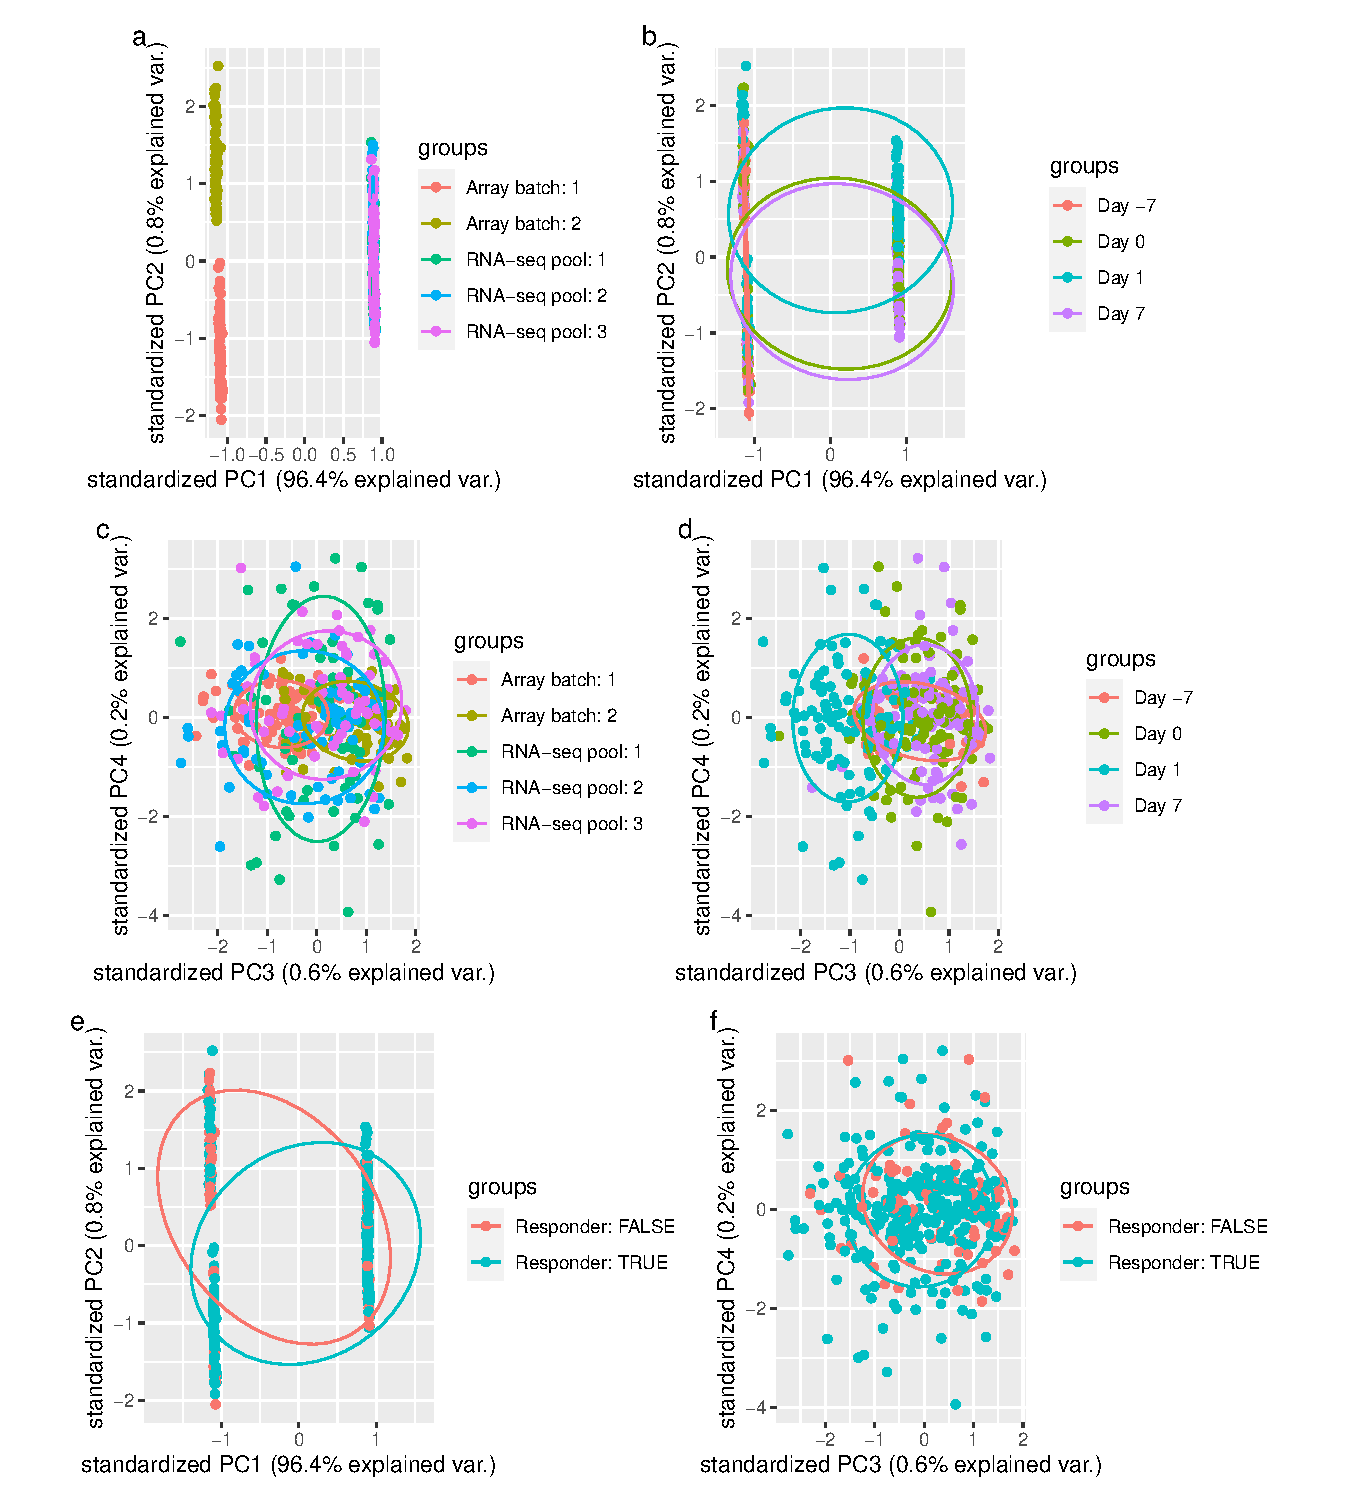
\includegraphics[width=1.0\textwidth,page=1]{mainmatter/figures/chapter_02/compare_phenotype_by_platform.E_pca.pdf}
    \caption{First 2 expression PCs, expressions first standardized within platform to increase comparability, if not, even more variation would be driven by platform}
    \label{fig:hird_expression_pcs}
\end{figure}

% Also see: https://support.bioconductor.org/p/72815/
Regarding the batch effect within the \gls{HIRD} array data, a popular adjustment method is ComBat\autocite{johnson2007AdjustingBatchEffects}, which estimates centering and scaling parameters per-gene pooling information across all genes using empirical Bayes.
ComBat is the method used in \autocite{sobolev2016AdjuvantedInfluenzaH1N1Vaccination}.
In comparisons of microarray batch effect adjustment methods, ComBat performs favourably (vs. five other adjustment packages)\autocite{chen2011RemovingBatchEffects} or comparably (vs. batch as a fixed or random effect in the linear model)\autocite{espin-perez2018ComparisonStatisticalMethods}.
However, where batches are unbalanced in terms of sample size\autocite{zhang2018AlternativeEmpiricalBayes} or distribution of study groups that have an impact on expression\autocite{nygaard2015MethodsThatRemove}, ComBat can overcorrect batch differences or bias estimates of group differences respectively.
In our data, sample size and timepoint groups are fairly balanced between the two array batches, but the proportion of responders is not\autoref{tab:hird_batch_balance}, hence I elect not to use ComBat to pre-adjust the array expression data, and model the batches as fixed effects.
In practice, results from the \gls{DGE} analysis were not substantially affected by the choice of whether to use a ComBat pre-adjustment or a fixed effect.
\todo{this is not a very precise justification. actually, if I were to color R/NR in the PCA plot, R/NR doesn't really explain a lot of var in global gene expression. that's probably why the results don't change much. then the justification can be simplicity. should probably do this at some point.}

\begin{table}[] 
 \centering 
 \caption[\captionshort{Distribution of \gls{HIRD} samples among timepoint and responder groups in the array batches and \gls{RNAseq} pools.}]{\textbf{Distribution of \gls{HIRD} samples among timepoint and responder groups in the array batches and \gls{RNAseq} pools.} Values are count and percentage for categorical variables; mean and standard deviation for continuous variables.}\label{tab:hird_batch_balance}
 \begin{tabular}{ l c c c c c c }
 \toprule
  &   &  \multicolumn{ 5 }{c}{ Array batch/\gls{RNAseq} pool }\\ 
  & Total & Array 1 & Array 2 & \gls{RNAseq} 1 & \gls{RNAseq} 2 & \gls{RNAseq} 3\\ 
  & n = 374 & n = 87 & n = 79 & n = 70 & n = 69 & n = 69 \\ 
  \midrule
 Day &   &   &   &   &   &  \\ 
 \hspace{6pt}    -7 & 40 (10.7\%) & 20 (23\%) & 20 (25.3\%) & 0 (0\%) & 0 (0\%) & 0 (0\%)\\ 
 \hspace{6pt}    0 & 114 (30.5\%) & 24 (27.6\%) & 20 (25.3\%) & 24 (34.3\%) & 23 (33.3\%) & 23 (33.3\%)\\ 
 \hspace{6pt}    1 & 109 (29.1\%) & 21 (24.1\%) & 20 (25.3\%) & 22 (31.4\%) & 23 (33.3\%) & 23 (33.3\%)\\ 
 \hspace{6pt}    7 & 111 (29.7\%) & 22 (25.3\%) & 19 (24.1\%) & 24 (34.3\%) & 23 (33.3\%) & 23 (33.3\%)\\ 
 Responder &   &   &   &   &   &  \\ 
 \hspace{6pt}    FALSE & 80 (21.4\%) & 12 (13.8\%) & 36 (45.6\%) & 11 (15.7\%) & 9 (13\%) & 12 (17.4\%)\\ 
 \hspace{6pt}    TRUE & 294 (78.6\%) & 75 (86.2\%) & 43 (54.4\%) & 59 (84.3\%) & 60 (87\%) & 57 (82.6\%)\\ 
 TRI &   &   &   &   &   &  \\ 
 \hspace{6pt}   & -0.1 (1.0) & -0.1 (1.0) & -0.4 (1.4) & 0.1 (0.6) & -0.0 (0.8) & 0.2 (0.6)\\ 
 \bottomrule
 
 \end{tabular}
 \end{table}


\subsubsection{Per-platform \glsfmtlong{DGE} model}

% Also used arrayWeights as precision weight inputs to lmFit
% See: https://bmcbioinformatics.biomedcentral.com/articles/10.1186/1471-2105-7-261#Bib1
% The method successfully assigns lower weights to less reproducible arrays from different experiments. Down-weighting the observations from suspect arrays increases the power to detect differential expression.
As \autocite{sobolev2016AdjuvantedInfluenzaH1N1Vaccination} demonstrated no significant global difference in array expression between day -7 and day 0, I likewise treat merge these two timepoints into a single baseline timepoint \enquote{day 0} in the following \gls{DGE} models.

% 5.6.	Between-sample normalization of library size: Trimmed mean of M-values (TMM)
% Selecting between-sample RNA-Seq normalization methods from the perspective of their assumptions https://www.ncbi.nlm.nih.gov/pmc/articles/PMC6171491/
% 5.6.1.	edgeR::calcNormFactors generates norm.factors for each sample
For \gls{RNAseq} samples, between-sample normalisation was performed using the \gls{TMM} method\autocite{evans2018SelectingBetweensampleRNASeq} from edgeR\autocite{robinson2010EdgeRBioconductorPackage}; 
then variance-stabilisation was performed using voom\autocite{law2014VoomPrecisionWeights}, resulting in expression values with units of $\log_2{\text{\gls{CPM}}}$.

% 7.	Differential expression (limma)
% 7.2.	Create contrasts
% 7.3.	Estimate within-block correlation (duplicateCorrelation), using patients as blocks
% 7.4.	Array data only: Compute sample quality weights for each array (arrayWeightsSimple(v, design=mod1))
% 7.5.	RNA-seq data only: Correct for mean-variance trend (voom)
% 7.5.1.	http://web.mit.edu/~r/current/arch/i386_linux26/lib/R/library/limma/html/voom.html
% 7.5.1.1.	“voom is an acronym for mean-variance modelling at the observational level. The key concern is to estimate the mean-variance relationship in the data, then use this to compute appropriate weights for each observation. Count data almost show non-trivial mean-variance relationships. Raw counts show increasing variance with increasing count size, while log-counts typically show a decreasing mean-variance trend. This function estimates the mean-variance trend for log-counts, then assigns a weight to each observation based on its predicted variance. The weights are then used in the linear modelling process to adjust for heteroscedasticity.”
% 7.5.1.2.	“voom performs the following specific calculations. First, the counts are converted to logCPM values, adding 0.5 to all the counts to avoid taking the logarithm of zero. The matrix of logCPM values is then optionally normalized. The lmFit function is used to fit row-wise linear models. The lowess function is then used to fit a trend to the square-root-standard-deviations as a function of average logCPM. The trend line is then used to predict the variance of each logCPM value as a function of its fitted value, and the inverse variances become the estimated precision weights.”
% 7.6.	(lmFit)
% 7.7.	(contrasts.fit)
% 7.8.	(eBayes/treat)
% 7.8.1.1.1.	https://rdrr.io/bioc/limma/man/ebayes.html
% 7.8.1.1.1.1.	When lfc=0, treat is identical to eBayes, except that F-statistics and B-statistics are not computed.
% 7.8.1.1.2.	https://academic.oup.com/bioinformatics/article/25/6/765/251641 The TREAT fold-change threshold should be set to a low value below which no fold-change is likely to be of genuine interest. Researchers should be mindful that genes will need to exceed this threshold by some way, depending on the data, before being declared statistically significant. Our experience suggests a minimal value, such as a 10% fold-change, corresponding to τ=log2(1.1)=0.13 on the log2-scale. It would be better to interpret the threshold as ‘the fold-change below which we are definitely not interested in the gene’ rather than ‘the fold-change above which we are interested in the gene’.
% 7.9.	(decideTests)
Linear models were fit using limma\autocite{ritchie2015LimmaPowersDifferential}, which is computationally fast, and performs well for sufficiently large ($n \ge 3$ per group) samples\autocite{soneson2013ComparisonMethodsDifferential}
For each gene, I fit a model (model 1) with expression as the response; and timepoint (baseline, day 1, day 7), \gls{TRI}, batch, sex, age, and the first 4 genotype \glspl{PC} as fixed-effect predictors; and individual as a random-effect predictor.
\todo{link to papers justifying sex, age, ancestry as significant effects on immune gene expression}
Within-individual correlations for the random effect were estimated using limma::duplicateCorrelation.
A second model (model 2) was also fit, including 3 additional terms for the interactions between each timepoint and \gls{TRI}.
% https://support.bioconductor.org/p/70175/
% es <- fit2$coefficients
% es_se <- sqrt(fit2$s2.post) * fit2$stdev.unscaled
Coefficients and their standard errors were extracted from the linear models.\todo{specify which particular contrasts are extracted from which model}
These coefficients represent effect size in units of log2 expression fold-change per unit change in predictor value.

\subsubsection{Choice of \glsfmtlong{DGE} meta-analysis method}

In the section \todo{add section labels}, I concluded that a two-stage meta-analysis approach would be appropriate.
This meta-analysis is restricted to 13593 genes assayed by both the array and \gls{RNAseq} platforms.
% While there is abundant literature on single-plaform (e.g. \autocite{tseng2012ComprehensiveLiteratureReview}) methods [...]
%
% Examples from literature
%
% random effects:
%
% https://academic.oup.com/nar/article/45/17/9860/4084660#106485896
% - for example of REM of 24 array datasets
%
% Sweeney, T. E., Haynes, W. A., Vallania, F., Ioannidis, J. P., & Khatri, P. (2017). Methods to increase reproducibility in differential gene expression via meta-analysis. Nucleic Acids Research, 45(1), e1–e1. https://doi.org/10.1093/nar/gkw797
% - DGE random effects models should be possible with around 6-7 studies.
%
% SVA:
% Comparative RNA-Seq and Microarray Analysis of Gene Expression Changes in B-Cell Lymphomas of Canis familiaris
% https://www.ncbi.nlm.nih.gov/pmc/articles/PMC3617154/
% - applying SVA to our data revealed a strong correlation with known technical biases associated with RNA-Seq [26]–[28], [51] and removing the associated variation from the RNA-Seq samples resulted in the two technologies pairing by individual sample.
% - First, we have not attempted to capture differences in dynamic range between RNA-Seq and microarray. It is reasonable to expect that the larger dynamic range of RNA-Seq will result in larger variation. We found latent variation to be highly associated with GC content but, in contrast, found no clear evidence of an association pointing to nonlinear response in the microarrays. Second, the model underlying SVA does not explicitly capture different latent variables for the different technologies.
%
% MetaVolcano:
% The MetaVolcanoR R package combines differential gene expression results. It implements three strategies to summarize gene expression activities from different studies. i) Random Effects Model (REM) approach. ii) a vote-counting approach, and iii) a p-value combining-approach.
% - doesn't solve our small k problem
%
% CorMotif:
% https://academic.oup.com/biostatistics/article/16/1/31/259492
% - In contrast, a model that naively enumerates and analyzes all possible differential patterns across studies can deal with study-specificity and allow information pooling, but the complexity of its parameter space grows exponentially as the number of studies increases.
% - Here, we propose a correlation motif approach to address this dilemma. This approach searches for a small number of latent probability vectors called correlation motifs to capture the major correlation patterns among multiple studies.
% - First applies limma (Smyth, 2004) to each study separately. CorMotif is made for microarray data since it was motivated by the microarray analysis in the Sleep for Health in Hospital Programme (SHH) study. However, the idea behind CorMotif is general, and it should be straightforward to develop a similar framework for RNA-seq data.
% - designed for large k, seems similar to mashr
%
% CBM (“Cross-platform Bayesian Model”):
% - In this article, we propose a Bayesian hierarchical model to jointly integrate microarray and RNA-seq studies.
% - Since systematic fold change differences across RNA-seq and microarray for detecting differentially expressed genes have been previously reported, we replicated this finding in several real datasets and showed that incorporation of a normalization procedure to account for the bias improves the detection accuracy and power.
% - Cannot acually use CBM, as it operates on expressions, with a binary case vs control, so no covariates
%
% RankProd:
% - The Bioconductor package RankProd provides a new and intuitive tool for this purpose in detecting differentially expressed genes under two experimental conditions.
%
% Mayday seasight:
% - Uses a rank product model internally

Two popular frameworks for effect size meta-analysis are fixed-effect and random-effects\autocite{cohn2003HowMetaanalysisIncreases,borenstein2010BasicIntroductionFixedeffect}.
Given k studies, the fixed-effect model assumes a common population effect size shared across all studies, with observed variation explained only by sampling error.
The random-effects model assumes the k study-specific effect sizes are drawn from some distribution with variance $\tau^2$ (\gls{SD} $\tau$), representing an additional source of variation termed the between-studies heterogeneity, reducing to the fixed-effect model when $\tau=0$
In the \gls{HIRD} data, there are $k=2$ 'studies' (array and \gls{RNAseq}), where the platform differences described in section\todo{add label} contribute to between-studies heterogeneity, the assumption of $\tau=0$ is unrealistic, hence a random-effects model is more appropriate.
\todo{make all the notation in this section consistent with, and add the equation 2.1. The normal-normal hierarchical model, \autocite{rover2017BayesianRandomeffectsMetaanalysis}}

Unfortunately, there is no optimal solution for directly estimating $\tau$ in random-effects meta-analyses with small k\autocite{bender2018MethodsEvidenceSynthesis}, especially when $k=2$\autocite{gonnermann2015NoSolutionCombining}.
Many estimators are available\autocite{veroniki2016MethodsEstimateBetweenstudy}, but lack of information with small k causes estimation to be imprecise, and can often result in boundary values of $\tau = 0$ that are incompatible with the assumed positive heterogeneity\autocite{chung2013NondegeneratePenalizedLikelihood,friede2017MetaanalysisFewSmall}.
In such circumstances, the most sensible choice may be to incorporate prior information about model hyperparameters in a Bayesian random-effects framework\autocite{chung2013NondegeneratePenalizedLikelihood,veroniki2016MethodsEstimateBetweenstudy,friede2017MetaanalysisFewSmall,seide2019LikelihoodbasedRandomeffectsMetaanalysis}.
For this study, I use the implementation in bayesmeta \autocite{rover2017BayesianRandomeffectsMetaanalysis}, which requires priors for both effect size and between-studies heterogeneity.

\subsubsection{Prior for between-studies heterogeneity}

The choice of prior for between-studies heterogeneity is influential when k is small\autocite{seide2019LikelihoodbasedRandomeffectsMetaanalysis}.
\textcite{gelman2006PriorDistributionsVariance} considers the case of $k=3$, showing that a flat prior places too much weight on implausibly large estimates of $\tau$, and recommends a weakly informative prior that acts to regularise the posterior distribution.
% Gelman 
% - weak as in deliberately weaker than known knowledge, just serves to constrain
% - cauchy for the gentle slope in tails
% - also warns against inverse-gamma(e, e), as it can influence the posterior mean; it is not at all non-informative.
%
% Similarly, \autocite{friede2017MetaanalysisFewSmall} consider half-normals.
%
% More recent recommendations:
% \footnote{Documentation for Stan: \url{https://github.com/stan-dev/stan/wiki/Prior-Choice-Recommendations}.}
% - Gelman 2006 recommendations can actually be too weak for scale
% - Recommends Chung gamma(2, 1/A)
% - With full Bayes the boundary shouldn't be a problem (as long as you have any proper prior).
% - But with modal estimation, the estimate can be on the boundary, which can create problems in posterior predictions. For example, consider a varying-intercept varying-slope multilevel model which has an intercept and slope for each group. Suppose you fit marginal maximum likelihood and get a modal estimate of 1 for the group-level correlation. Then in your predictions the intercept and slope will be perfectly correlated, which in general will be unrealistic.
% Chung, Y., Rabe-Hesketh, S., Dorie, V., Gelman, A., & Liu, J. (2013). A Nondegenerate Penalized Likelihood Estimator for Variance Parameters in Multilevel Models. Psychometrika, 78(4), 685–709. https://doi.org/10.1007/s11336-013-9328-2
Since I assumed non-positive values for $tau$ are unrealistic, I use a weakly-informative gamma prior recommended by \autocite{chung2013NondegeneratePenalizedLikelihood}, which has zero density at $\tau = 0$, increasing gently as $\tau$ increases.
This constrains $\tau$ to be positive, but still permits estimates close to zero if the data support it.
This is in constrast to log-normal (e.g. \autocite{pullenayegum2011InformedReferencePrior,turner2015PredictiveDistributionsBetweenstudy}) or inverse-gamma priors (e.g. \autocite{higgins1996BorrowingStrengthExternal}) which have derivatives close to zero, and rule out small values of $tau$ no matter what the data suggest; and in contrast to half-t family priors (e.g. \autocite{gelman2006PriorDistributionsVariance,seide2019LikelihoodbasedRandomeffectsMetaanalysis}), which have their mode at zero, and do not rule out $tau=0$.

% rma.uni function
% By default, the starting value is set equal to the value of the Hedges (HE) estimator and the algorithm terminates when the change in the estimated value of \tau2 is smaller than 10^-5 from one iteration to the next.
To estimate the appropriate shape and scale parameters for the gamma empirically, a random-effects model using the \gls{REML} estimator for $\tau$ (recommended for continuous effects\autocite{veroniki2016MethodsEstimateBetweenstudy}) was first for each gene using \texttt{metafor}.
Genes with small estimates of $\tau < 0.01$ were excluded, and a gamma distribution was fit to the remaining estimates using \texttt{fitdistrplus}.

\subsubsection{Prior for effect size}

While the choice of prior on $\tau$ is influential when k is small, there is usually enough data to estimate the effect size $\mu$ such that any reasonable non-informative prior can be used \autocite{gelman2006PriorDistributionsVariance,friede2017MetaanalysisFewSmall} \todo{why is this? is it having well powered studies? gelman is vague}
\texttt{bayesmeta} implements both flat and normal priors for $\mu$.


% https://github.com/stan-dev/stan/wiki/Prior-Choice-Recommendations
% For example, it is common to expect realistic effect sizes to be of order of magnitude 0.1 on a standardized scale (for example, an educational innovation that might improve test scores by 0.1 standard deviations). In that case, a prior of N(0,1) could be considered very strong, in that it puts most of its mass on parameter values that are unrealistically large in absolute value. When we say this prior is "weakly informative," what we mean is that, if there's a reasonably large amount of data, the likelihood will dominate, and the prior will not be important. If the data are weak, though, this "weakly informative prior" will strongly influence the posterior inference. The phrase "weakly informative" is implicitly in comparison to a default flat prior.
% Weakly informative prior should contain enough information to regularize: the idea is that the prior rules out unreasonable parameter values but is not so strong as to rule out values that might make sense
% Weakly informative rather than fully informative: the idea is that the loss in precision by making the prior a bit too weak (compared to the true population distribution of parameters or the current expert state of knowledge) is less serious than the gain in robustness by including parts of parameter space that might be relevant. It's been hard for us to formalize this idea.
% One principle: write down what you think the prior should be, then spread it out. The idea is that the cost of setting the prior too narrow is more severe than the cost of setting it too wide. I've been having trouble formalizing this idea.
% Don't use uniform priors, or hard constraints more generally, unless the bounds
% represent true constraints (such as scale parameters being restricted to be
% positive, or correlations restricted to being between -1 and 1).
Assuming that most genes are not differentially expressed with effect sizes distributed randomly around zero, I choose a very weak normal prior with $\mu=0$ over a flat prior.

As in the section above, to get the appropriate scale, a normal distribution with mean $\mu = 0$ is fit to the distribution of effect sizes from the gene-wise metafor models to empirically estimate the \gls{SD} $\sigma$.
% Another Cauchy example:
% Gelman, A., Jakulin, A., Pittau, M. G., & Su, Y.-S. (2008). A weakly informative default prior distribution for logistic and other regression models. The Annals of Applied Statistics, 2(4), 1360–1383. https://doi.org/10.1214/08-AOAS191
% - Cauchy 2.5
Heavy-tailed Cauchy priors have been proposed for effect size distributions in \gls{DGE} experiments to avoid over-shrinkage of large effects\autocite{zhu2019HeavytailedPriorDistributions}.
Since \texttt{bayesmeta} does not implement a Cauchy prior, the normal prior used for meta-analysis is flattened to $N(0, 10\sigma)$ to avoid over-shrinkage in the tails.
This prior is equivalent to assuming a 95\% probability that effects are less extreme than approximately $20\sigma$.\todo{the derivation here is qnorm(0.975, mean=0, sd=1*10) = 1*19.59964}

\subsubsection{Evaluation of priors}

\autocite{chung2013NondegeneratePenalizedLikelihood} recommends (shape=2, scale=$\lambda$), with small $\lambda$.
\todo{From \autoref{fig:hird_dgeMeta_priors_tau} we are similar.}

\begin{figure}
    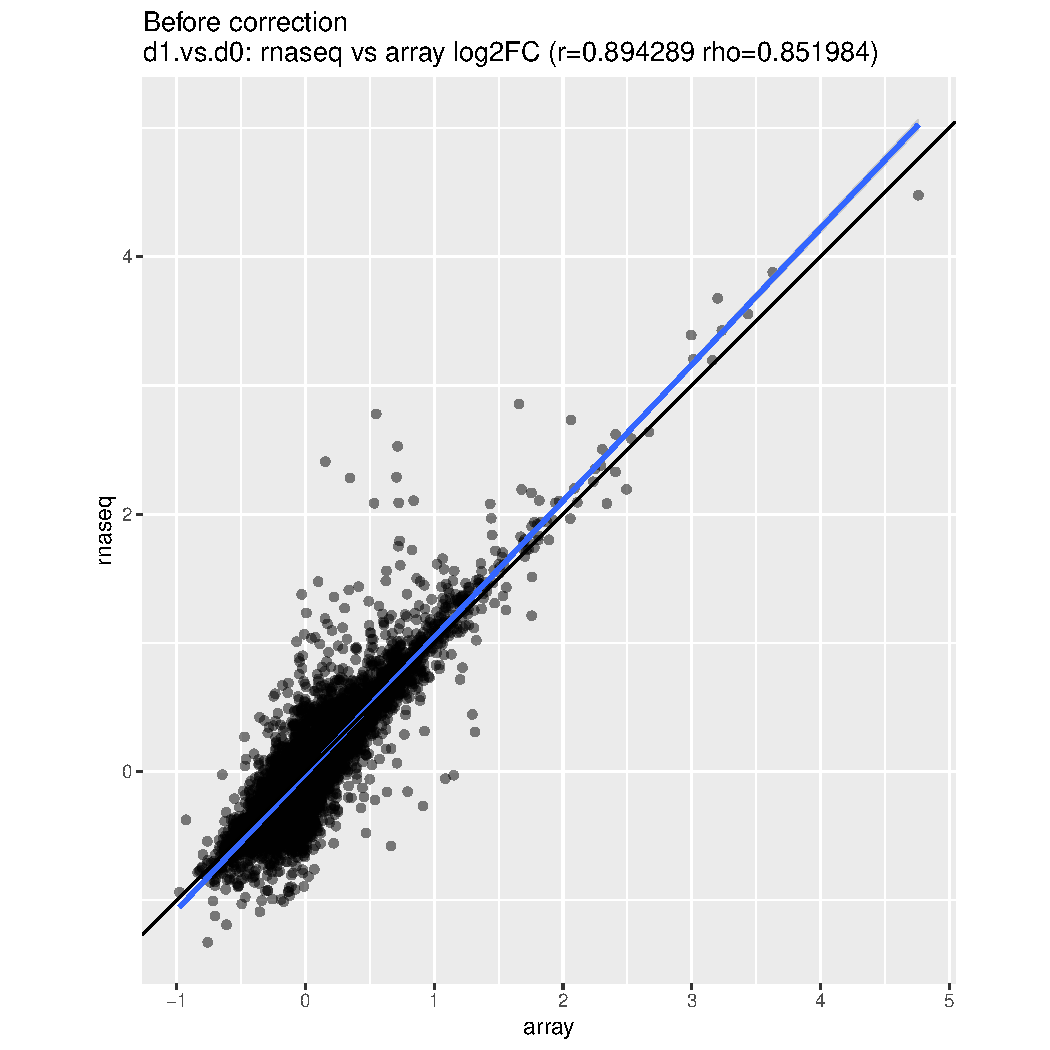
\includegraphics[width=1.0\textwidth]{mainmatter/figures/chapter_02/meta.rnaseqVsArray.log2FC.beforeBiasCorrection.coefName_d1.vs.d0.pdf}
    \caption{Fold-change comparison between array and RNAseq for day 1 vs day 0.}
    \label{fig:hird_dgeMeta_fcComparison}
\end{figure}

\begin{figure}
    \includegraphics[width=1.0\textwidth,page=2]{mainmatter/figures/chapter_02/meta.bayesmeta.priors.coefName_d1.vs.d0.pdf}
    \caption{Priors for tau for day 1 vs day 0 DGE meta-analysis.}
    \label{fig:hird_dgeMeta_priors_tau}
\end{figure}

\begin{figure}
    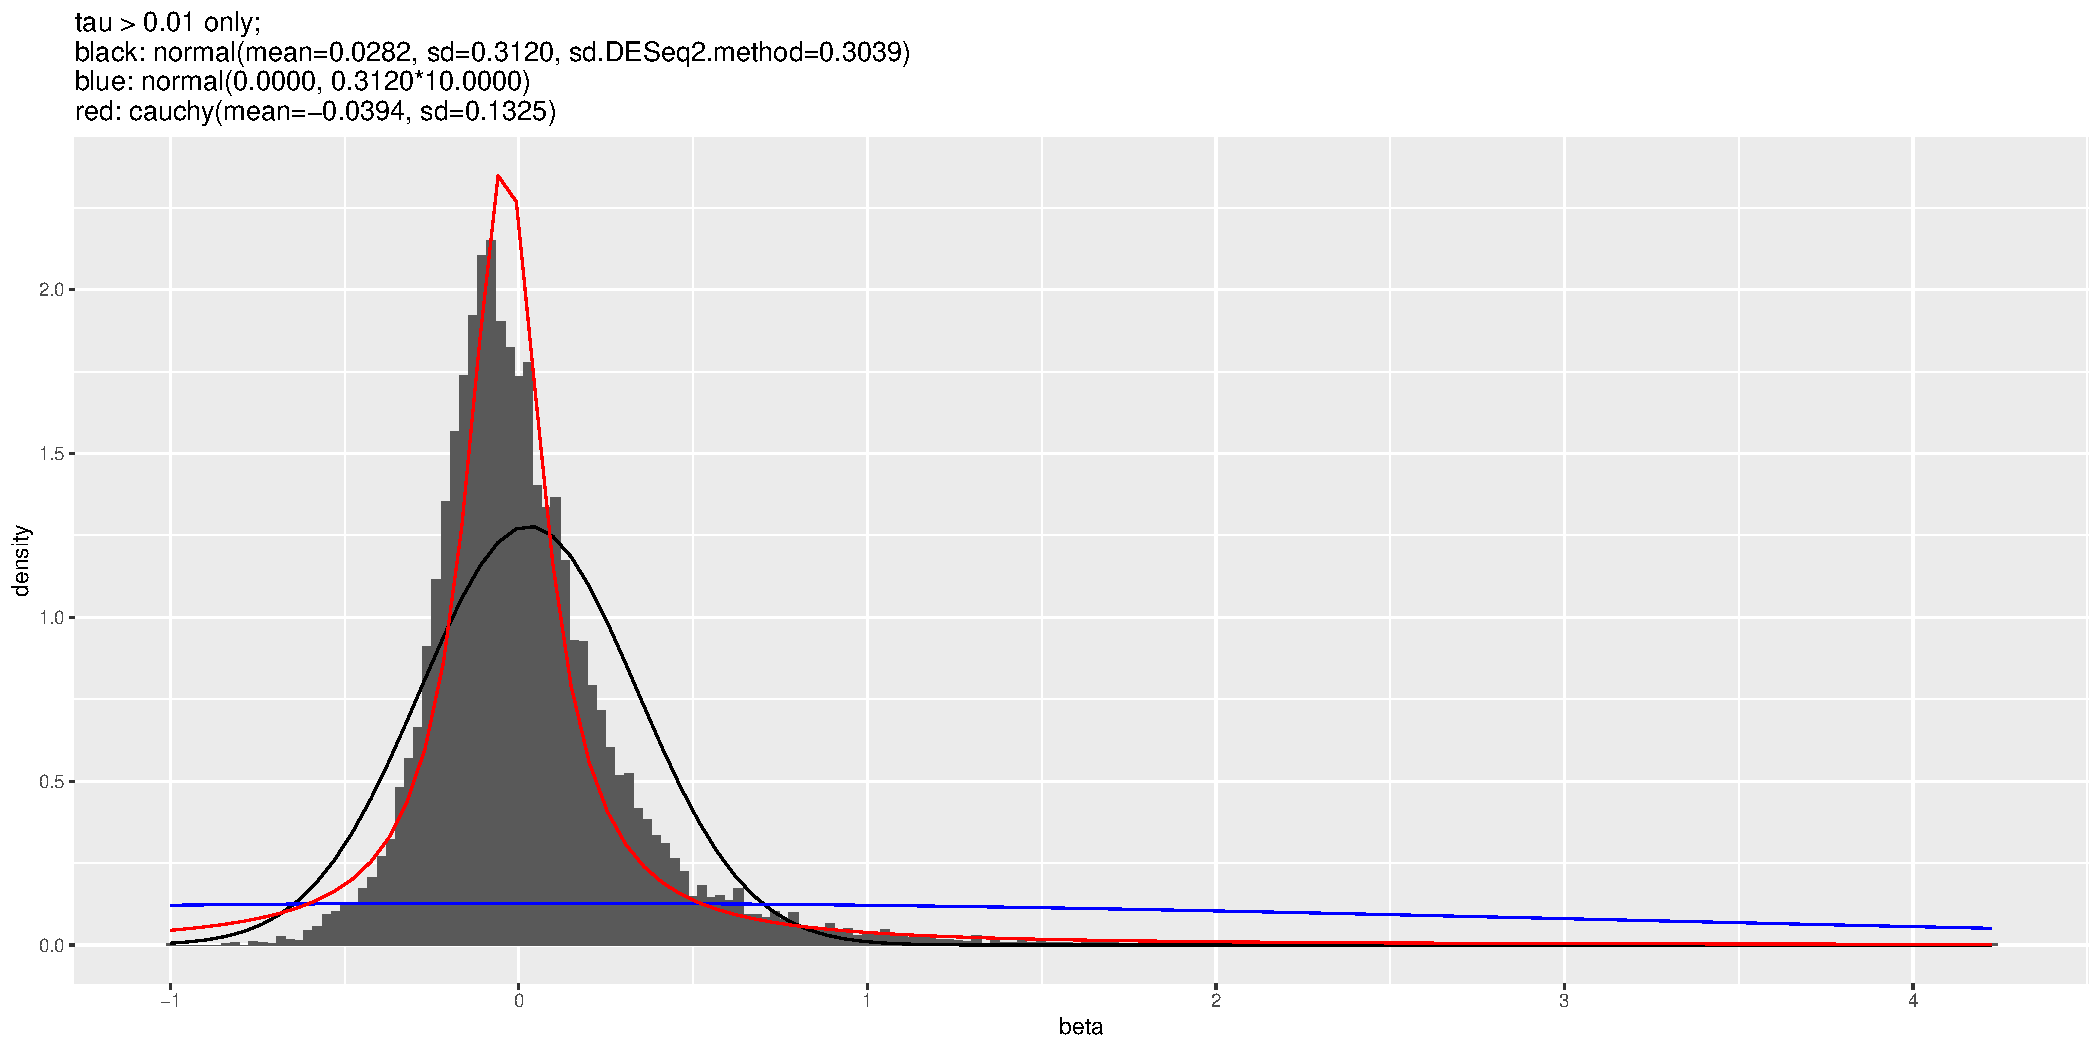
\includegraphics[width=1.0\textwidth,page=1]{mainmatter/figures/chapter_02/meta.bayesmeta.priors.coefName_d1.vs.d0.pdf}
    \caption{Priors for mu for day 1 vs day 0 DGE meta-analysis.}
    \label{fig:hird_dgeMeta_priors_mu}
\end{figure}

\subsubsection{FDR}

\todo{ashr}

% bayesmeta
% Posterior predictive checks are implemented in the pppvalue() to generate pvalues by MCMC.
% Do not confuse with ma05$pposterior(mu=0), which is evaluation of the posterior distribution at a particular value.

\subsection{Gene set enrichment analysis}

\todo{tmod; gprofileR; CAMERA}

\section{Results}

\subsection{Extensive global changes in expression after vaccination}

To gain an overview of how the transcriptome changes after vaccination, linear models were fit to identify genes differentially expressed at day 1 or day 7 compared to baseline (day -7 and day 0) in the \gls{HIRD} array and \gls{RNAseq} expression data, accounting for covariates such as batch effects, sex, age, \gls{TRI}, and ancestry.
At 13593 genes with expression measured by both platforms, models were fit within each platform, then effect sizes were combined using Bayesian random-effects meta-analysis.

At a \gls{lfsr}$ < 0.05$ and absolute $\text{fold change} > 1.5$ cutoff, 857/13593 genes were differentially expressed between any pair of timepoints.
Clustering the expression of these genes revealed three main clusters: 692 genes that tend to be upregulated at day 1, 94 gene upregulated at day 7, and 59 genes downregulated at day 1 (\autoref{fig:hird_dge_heatmap}).
 
\begin{figure}
    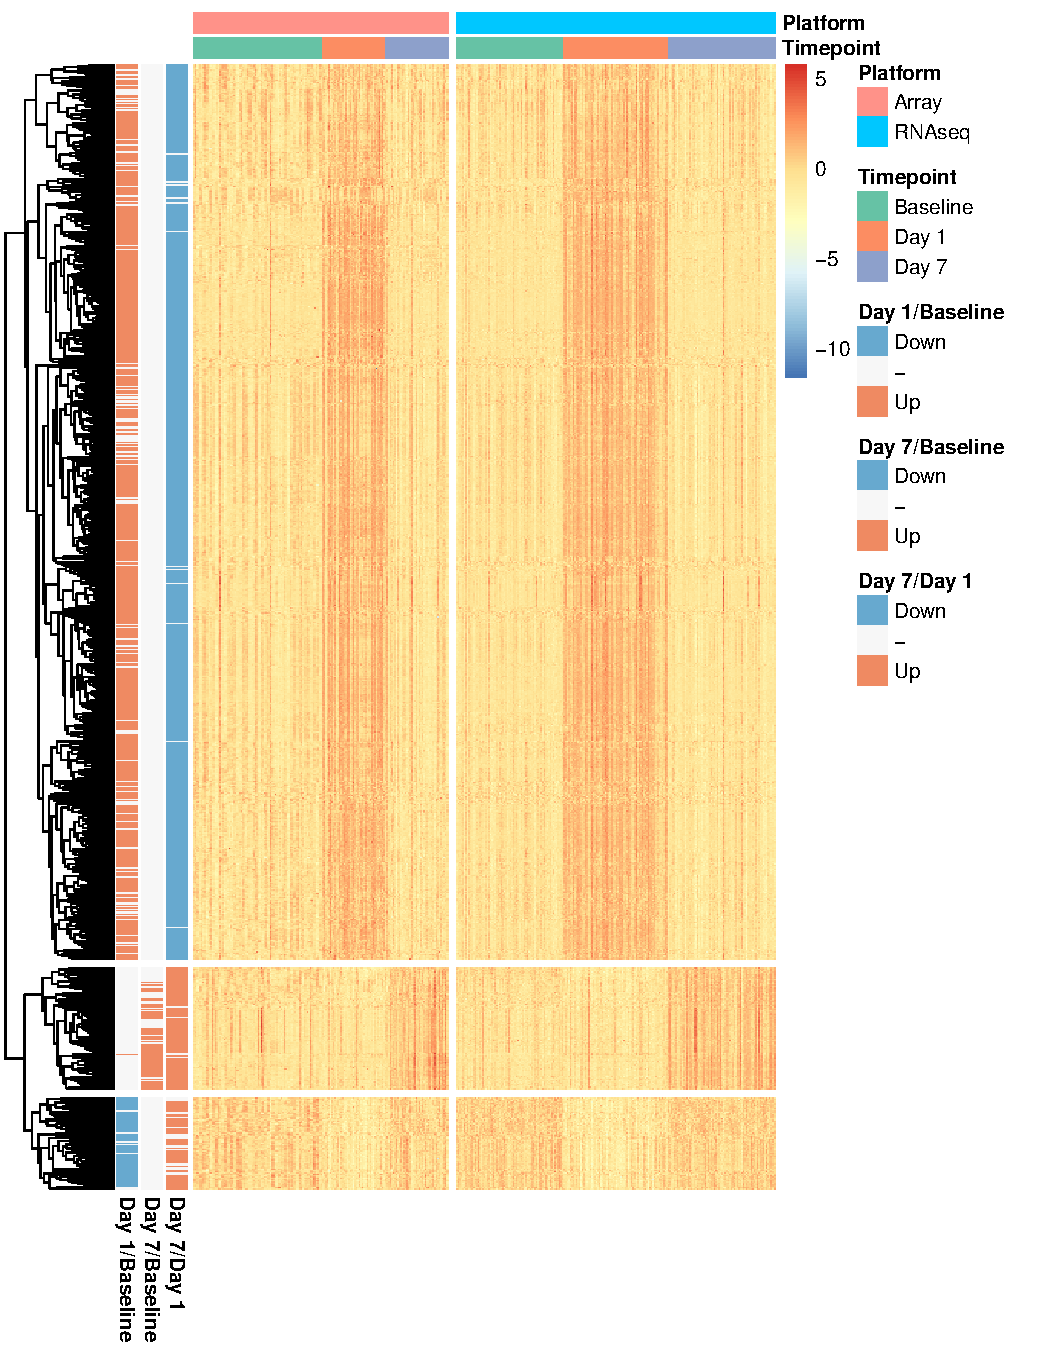
\includegraphics[width=1.0\textwidth]{mainmatter/figures/chapter_02/plot_dge_eqtl.heatmap_dge.pdf}
    \caption{Normalised gene expression for genes differentially expressed between any pair of timepoints ($\text{lfsr} < 0.05$, $\left|\text{FC}\right| > 1.5$) across \gls{HIRD}, clustered by gene. Distance metric: Manhattan.}
    \label{fig:hird_dge_heatmap}
\end{figure}

\subsection{Innate immune response at day 1 post-vaccination}

Consistent with global expression at day 1 being markedly different from expression at other timepoints (\autoref{fig:hird_expression_pcs}), the highest numbers of differentially expressed genes are observed at day 1, with 580 genes differentially expressed vs. baseline, the majority of which return to baseline by day 7.
The gene with the highest \gls{FC} increase at day 1 compared to baseline was \textit{ANKRD22} ($\log_2\text{\gls{FC}} = \num{4.489150}$), an interferon-induced gene in monocytes and \glspl{DC} involved in antiviral innate immune pathways\autocite{bin2016AnkyrinRepeatDomain}.
Other key genes in the interferon signalling pathway\autocite{schneider2014InterferonStimulatedGenesComplex} such as \textit{STAT1} ($\log_2\text{\gls{FC}} = 2.1693060$), \textit{STAT2}   ($\log_2\text{\gls{FC}} = 0.9489341$), and \textit{IRF9} ($\log_2\text{\gls{FC}} = 0.8153674$) are also upregulated at day 1.
Gene set enrichment analysis using \texttt{tmod} revealed that genes with the high \gls{FC} increases at day 1 were enriched in modules associated with activated \glspl{DC}, monocytes, toll-like receptor and inflammatory signalling (\autoref{fig:hird_tmodDotPlot_timepoint}), confirming that day 1 responses are dominated by signatures of innate immunity.
\todo{Not sure if there is a biological interpretion of downreg of T cells and NK cells gene sets, since it could be due to increase in other cell types in the sample}
\todo{any point in a table of e.g. top 20 DE genes, or is the gene set analysis already enough?}
\todo{can also add MSigDB hallmark sets, which include interferon sets; and of course gene ontology sets}

\begin{figure}
    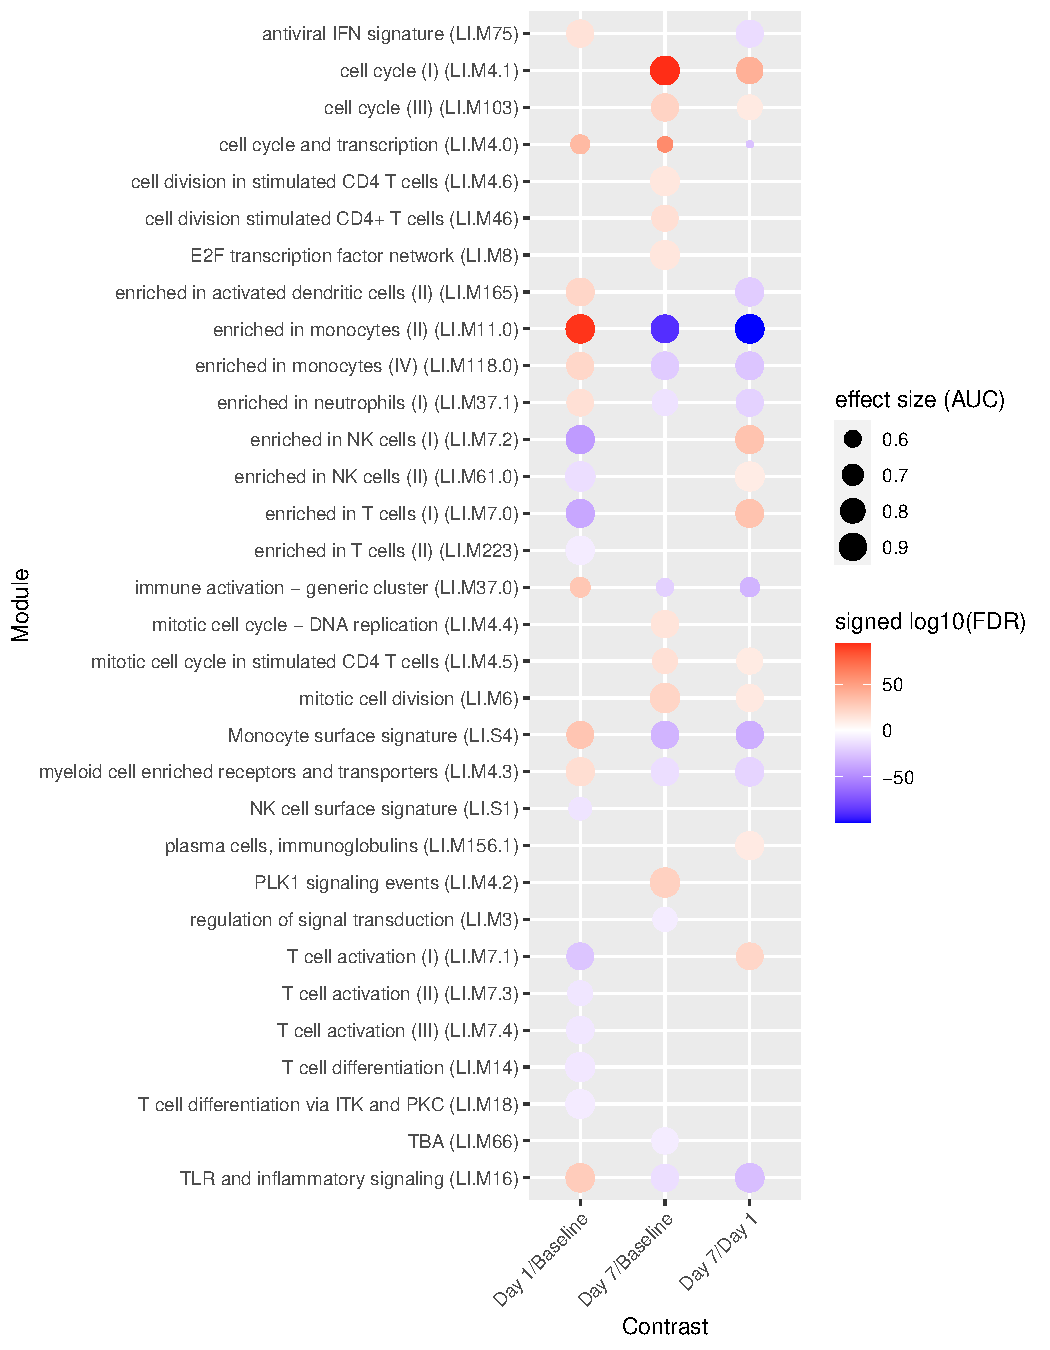
\includegraphics[width=1.0\textwidth]{mainmatter/figures/chapter_02/compare_dge_eqtl.tmodDotPlot.DGE.timepoint.pdf}
    \caption{Transcriptomic modules significantly up or downregulated post-vaccination. Size of circle indicates effect size. Color of circle indicates significance and direction of effect (red = upregulation, blue = downregulation).}
    \label{fig:hird_tmodDotPlot_timepoint}
\end{figure}
\todo{change x axis labels to baseline, specify top 10 procedure in figure caption}

\subsection{Adaptive immune response at day 7 post-vaccination}

Expression fold changes were more modest at day 7; the genes with the highest upregulation being the B cell-associated genes \textit{TNFRSF17} ($\log_2\text{\gls{FC}} = 1.7538617$) and \textit{MZB1} ($\log_2\text{\gls{FC}} = 1.7369668$).
Plasma cell-specific genes including \textit{SDC1} (encodes CD138 \url{https://www.ncbi.nlm.nih.gov/pmc/articles/PMC5437827/}) ($\log_2\text{\gls{FC}} = 1.3673081$) and \textit{ELL2} (\url{https://www.nature.com/articles/ni.1786}) ($\log_2\text{\gls{FC}} = 0.8679659$) were also prominently upregulated.
The enriched gene sets at day 7 were related to mitosis and cell proliferation, particularly in CD4\textsuperscript{+} T cells (\autoref{fig:hird_tmodDotPlot_timepoint}).
Both the CD4\textsuperscript{+} T cell and plasma cell response are indications of an adaptive immune response at day 7.
\todo{add reference to role of CD4s in e.g. class switching of B cells}

\subsection{Expression signatures associated with antibody response}

I also looked for genes which have expression associated with baseline-adjusted antibody response, as quantified by \gls{TRI}.
At the initial frequentist meta-analysis stage, with a significance threshold of FDR-BH $< 0.05$, 6 genes had expression associated with \gls{TRI} at day 0, 55 at day 7, and 11 pooled across timepoints (red, \autoref{fig:hird_DGE_effectSizeComparisons_rma}).
\autocite{sobolev2016AdjuvantedInfluenzaH1N1Vaccination} also identified genes with day 7 expression associated with antibody response, where response was defined as a binary phenotype based on 4-fold change (described in section \todo{add label}).
They reported 62 significant associations at \gls{FDR} $< 0.05$, of which 58/62 fall into the 13593 genes considered in my meta-analysis (circled, \autoref{fig:hird_DGE_platform_effectSizeComparisons_rma}), and 15/58 replicated, all with the same positive direction of effect (high expression correlates wtih high \gls{TRI}).
The Bayesian meta-analysis is more conservative.
No single gene was detected as significantly associated with \gls{TRI} at $\text{\gls{lfsr}} < 0.05$ at any timepoint, or when pooling samples across all timepoints (circled, \autoref{fig:hird_DGE_effectSizeComparisons_bayesmeta}).

\begin{figure}
    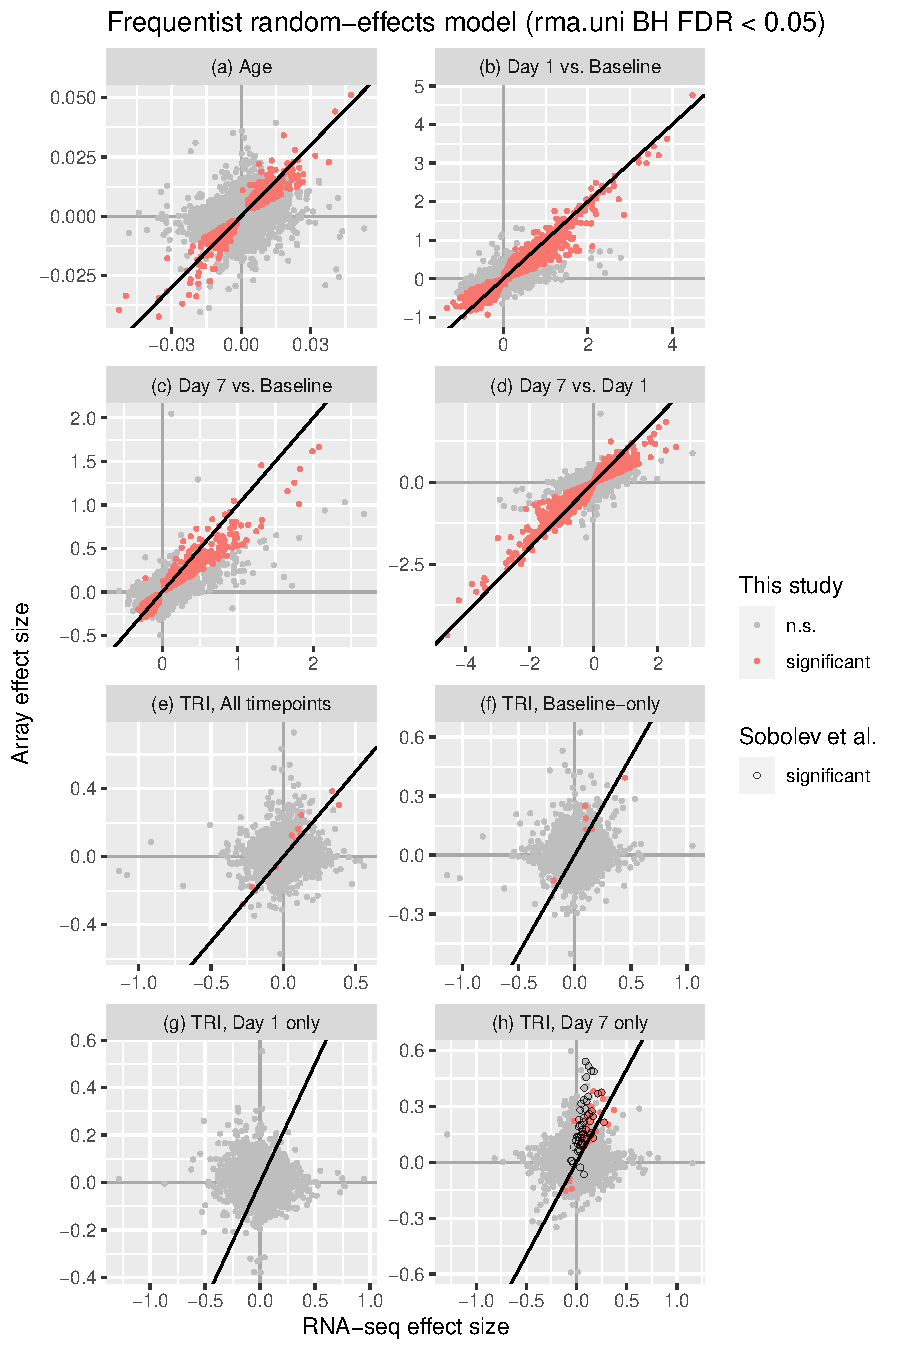
\includegraphics[width=1.0\textwidth,page=1]{mainmatter/figures/chapter_02/plot_dge_eqtl.DGE.effectSizeComparison.pdf}
    \caption{DGE effect sizes estimated in array vs \gls{RNAseq}. Significance colored by frequentist random effects meta-analyasis FDR < 0.05.}
    \label{fig:hird_DGE_effectSizeComparisons_rma}
\end{figure}

\begin{figure}
    \includegraphics[width=1.0\textwidth,page=2]{mainmatter/figures/chapter_02/plot_dge_eqtl.DGE.effectSizeComparison.pdf}
    \caption{DGE effect sizes estimated in array vs \gls{RNAseq}. Significance colored by Bayesian random effects meta-analysis lfsr < 0.05.}
    \label{fig:hird_DGE_effectSizeComparisons_bayesmeta}
\end{figure}

Significant enrichments can be detected at the gene set level; the strongest effects are seen at day 7, where expression of cell cycle, CD4\textsuperscript{+} T cells, and plasma cells are associated with high \gls{TRI}.
At day 0, modules related with inflammatory response in myeloid cells are also associated with high \gls{TRI} (\autoref{fig:hird_tmodDotPlot_TRI}).
\todo{have you explained how tmod works?}

\begin{figure}
    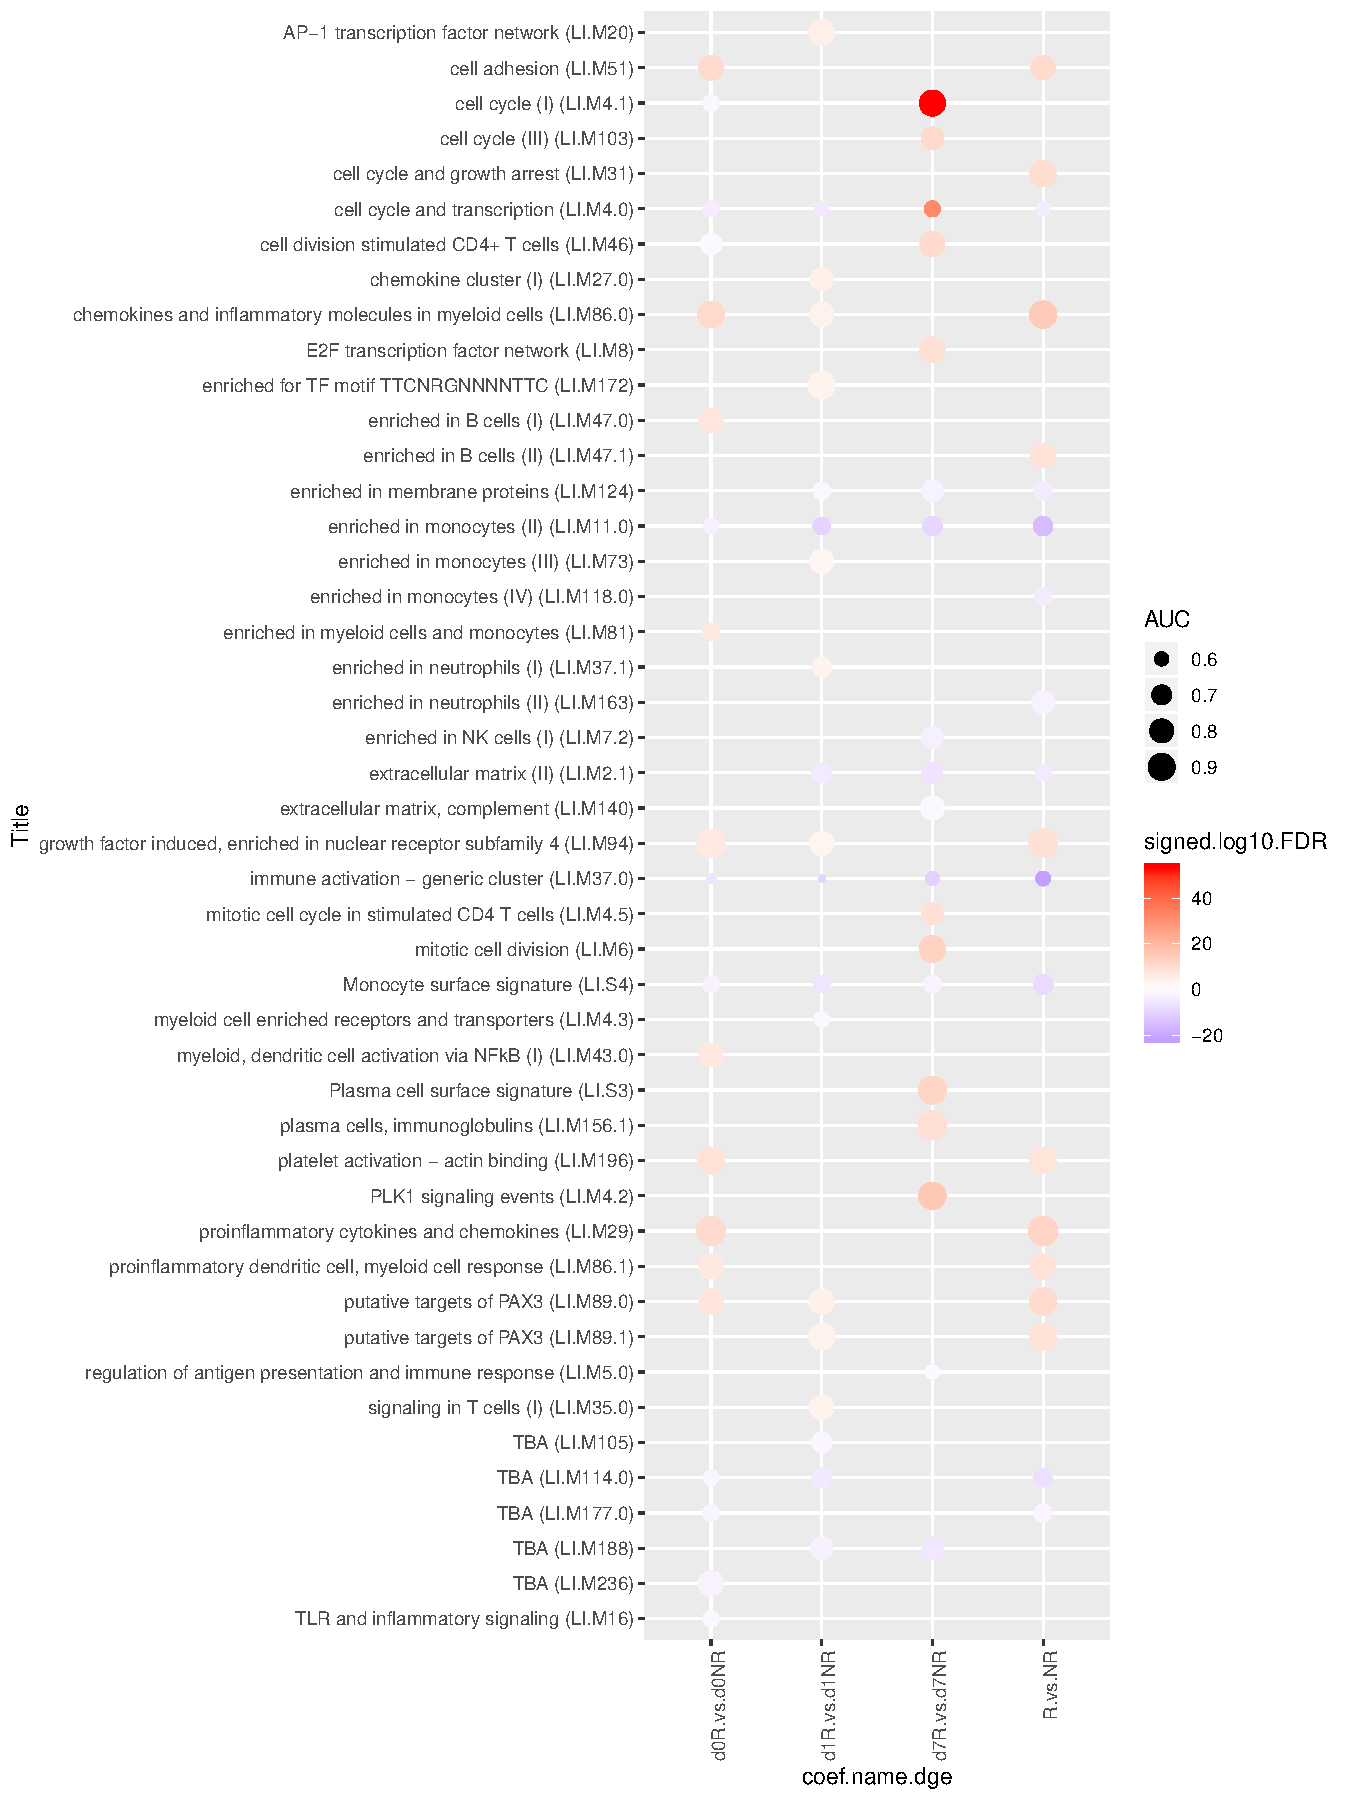
\includegraphics[width=1.0\textwidth]{mainmatter/figures/chapter_02/compare_dge_eqtl.tmodDotPlot.DGE.TRI.pdf}
    \caption{Transcriptomic modules enriched in genes with expression associated with antibody response (\gls{TRI}) at each day. Size of circle indicates effect size. Color of circle indicates significance and direction of effect (red = expression positively correlated with TRI, blue = negative).}
    \label{fig:hird_tmodDotPlot_TRI}
\end{figure}
\todo{figure x labels here should be TRI, not R.vs.NR}

\subsection{Identifying expression signatures for predicting antibody response}

\todo{analysis not complete, and possibly not even required for this chapter}

\section{Discussion}

% TODO: first thing to do is organise these commented paragraphs into the right order wrt existing points

% We have measured the transcriptomic response to influenza-H1N1 vaccination in the HIRD cohort, and characterised genes and gene sets differentially expressed between timepoints, and between vaccine responders/non-responders.
% Transient upregulation of many genes associated with interferons (a class of cytokines important for response to viral infection) and other aspects of innate immunity were detected at day 1, with most genes returning to baseline expression by day 7.
% Upregulation of immunoglobulin, B cell-related, and cell proliferation genes were detected at day 7---likely related to expansion of plasmablasts.
% Previous studies on seasonal influenza vaccines also reported induction of interferon-related genes 1-3 days post-vaccination, and enrichment of plasmablast and cell-cycle genes at day 7 \autocite{Nakaya2011, Franco2013, Nakaya2015a}.
%
% With regard to differential expression between the three timepoints, our results align with the microarray-based results of Sobolev et al.\autocite{Sobolev2016}, with similar trends in the relative numbers of DGEs for each comparison, and similar upregulation of interferon-inducible genes at day 1 (Fig.~\ref{fig-dge-interferons}).
% In addition, we also found differential expression at loci not present in the microarray.
%Top is ENSG00000173239	LIPM	protein_coding	10	1	-1.426	5.127	2.39e-11
% One such example was the gene with the highest fold-change increase from day 0 to day 1: LIPM (log2 FC = 5.127), a lipase implicated in epidermal barrier formation\autocite{Toulza2007}.
% We also detected upregulation of non-coding transcripts such as macrophage-associated\autocite{Zhang2017b} RP11-10J5.1.
% Compared to microarrays, which measure only at fixed number of probes, RNA-seq has the advantage of measuring transcriptome-wide, providing us more resolution when we come to build predictive models.
%and further investigation of these loci may be warrented, especially if they also form part of the predictive signatures themselves.
%
% In contrast, we failed to replicate DGE comparisons between responders and non-responders (Fig.~\ref{fig-dge-responders}).
% As we successfully replicated the timepoint DGE analyses, this is unlikely to be due purely to methodological differences, and more likely to be attributable to high variability within non-responders (i.e. ``many routes to failure''\autocite{Sobolev2016}).
% A different method for defining non-response may be required.
% Part of the variability within HIRD non-responders were `glass-ceiling' individuals with extremely high baseline antibody titres, making the four-fold increase required to be classified as a responder difficult to achieve\autocite{Sobolev2016}.
% We could consider using continuous measures of response corrected for baseline titre, such as the Titre Response Index\autocite{Bucasas2011}.
%Another advantage to using a continuous measure of vaccine response is the ability to define correlates? Not entirely sure though, since you could rank by p-value.
%
% Nevertheless, responders and non-responders in our dataset could still be distinguished; for example, gene sets related to TNFa/NFKb signalling (an important pathway in macrophages, dendritic cells and neutrophils\autocite{Liu2017}) and inflammatory response were upregulated in responders at all days.
% The fact that direction of response for many of the tested gene sets was consistent regardless of time after vaccination, even at day 0, suggests there may be factors that associate not with time post-vaccination, but rather are detectable even before vaccination.
% There is increasing evidence that these so called ``baseline predictors'' are identifiable in a variety of vaccines\autocite{Furman2013, Tsang2014, Nakaya2015a, HIPC-CHISignaturesProjectTeam2017}.
% A readily measurable variable prior to vaccination is genotype, but the contribution of genetic variation to forming baseline predictors is as yet unclear, due to the paucity of systems vaccinology studies that collect genetic data.

For inference, don't dichotimise due to statistical concerns
    % Nauta JJ, Beyer WE, Osterhaus AD. On the relationship between mean antibody level, seroprotection and clinical protection from influenza. Biologicals 2009; 37:216-21; PMID:19268607; http://dx. doi.org/10.1016/j.biologicals.2009.02.002
"In clinical studies seroprotection is normally defined as a specific antibody titer or antibody titer increase (seroconversion)."
For prediction, what rules can be easily implemented in the clinic?

Interpretatability: DAMIP gives rulesets composed of small sets of genes, amenable to rapid qPCR assays.


\begin{outline}
\1 Recap of results with limitations
% "Sobolev et al. identify an early interferon and lymphoid response that can be seen 1 day after vaccination2. These signals have not been detected in other studies, but this might be explained by differences in vaccine formulation. Specifically, the adjuvant might mimic the response pattern found to an attenuated virus6."
\1 Cannot directly separate adjuvant effect
\end{outline}

the day 63 timepoint is too late?
late compared to many other studies

Use hai and MN in split models
No change scores

other measures of seroconversion \url{https://www.who.int/biologicals/vaccines/Annex_2_WHO_TRS_963-3.pdf}

% https://bmcinfectdis.biomedcentral.com/articles/10.1186/s12879-019-4049-5
and seroconversion may not correspond well to protection...

day 7 most TRI association, as adaptive.
day 0 some association, more than day 1, suggests prevacc state is important

\subsection{Comparison to Sobolev R vs. NR}

\begin{outline}
\1 Differences between array-only and rnaseq-only DGE results for R/NR comparison (see 1st year report).

\1 Caveats of the meta analysis

what changes vs sobolev?
obviously, the TRI is not same as RvsNR

nonlinearity of effect
we do a meta, array vs rnaseq bias
two things: bayesmeta considers tau.
magnitudes of these effects are rather small
    given sufficient tau, will not be signif
68/72 have tau2=0 in the R.vs NR signifs.
second, fdr method is different
    Is the R vs NR bayesmeta -> lfsr method too stringent due to auto reg by a nice prior?
link to why usually not worry about multiple comps

Gene sets are more power

\end{outline}

\subsection{Inflammatory signatures of non-response}

% https://www.jacionline.org/article/S0091-6749(17)31766-9/fulltext#sec2.4
\enquote{The reduced efficacy of vaccination has also been linked to excessive inflammation for influenza,31 yellow fever,32 tuberculosis,33 and hepatitis B34 vaccines.}

Overall conclusions.
